\documentclass [12pt,letterpaper]{report}

% Standard packages
\usepackage{amsmath}		% Extra math definitions
\usepackage{graphics}		% PostScript figures
\usepackage{setspace}		% 1.5 spacing
\usepackage{longtable}          % Tables spanning pages
\DeclareGraphicsExtensions{.pdf,.png,.jpg,.mps}
\usepackage{amssymb}
\usepackage{mathtools}
\usepackage{ amsmath, bm }
\usepackage{graphicx}
\usepackage{epstopdf}
\usepackage{yhmath}
\usepackage{multirow}
\usepackage{longtable}
\usepackage{dsfont}
\usepackage{bbm}
\usepackage{float}
\usepackage[section]{placeins}


% Custom packages
\usepackage[first]{datestamp}	% Datestamp on first page of each chapter
\usepackage[fancyhdr]{McECEThesis}	% Thesis style
\usepackage{McGillLogo}		% McGill University crest

% $Id: ThesisEx.tex,v 1.1 2005/06/09 12:48:46 kabal Exp $

\usepackage{color}
\def\headrulehook{\color{red}}		% Color the header rule

%===== page layout
% Define the side margins for a right-side page
\insidemargin = 1.3in
\outsidemargin = 0.8in

% Above margin is space above the header
% Below margin is space below footer
\abovemargin = 1.1in
\belowmargin = 0.75in

\newcommand{\rmnum}[1]{\romannumeral #1}
\newcommand{\Rmnum}[1]{\expandafter\@slowromancap\romannumeral #1@}
\makeatother

\newcommand\bigfrown[2][\textstyle]{\ensuremath{%
  \array[b]{c}\text{\scalebox{2}{$#1\frown$}}\\[-1.3ex]#1#2\endarray}}

%========= Document start

\begin {document}

%===== Title page

\title{The Extended Neyman-Pearson Hypotheses Testing Framework and its Application to Spectrum Sensing in Cognitive Wireless Communication}
\author{An Jiang}
\date{\Month\ \number\year}
\organization{%
  \\[0.2in]
  \McGillCrest {!}{1in}\\	% McGill University crest
  \\[0.1in]
  Department of Electrical \& Computer Engineering\\
  McGill University\\
  Montreal, Canada}
\note{%
  {\color{red} \hrule height 0.4ex}
  \vskip 3ex
  A thesis submitted to McGill University in partial fulfillment of the
  requirements for the degree of Master of Engineering (M.Eng) in Electrical Engineering.
  \vskip 3ex
  \copyright\ \the\year\ An Jiang
}

\maketitle

%===== Justification, spacing for the main text
\raggedbottom
%\onehalfspacing
\doublespacing
\pagenumbering{roman}

%===== Abstract, Sommaire & Acknowledgments
\section*{\centering Abstract}
We propose a Modified Extended Neyman Pearson (MENP) framework which is suitable for spectrum sensing when there might be different types of primary signals. Our work generalizes existing Neyman Pearson (NP) test to multiple probability of false alarm constraints. This allows the cognitive radio wireless communication system to provide different levels of protection for various primary users.  
M-ROC surface, representing the relationship between the probability of detection and the constraints, is used to depict the performance of MENP testing.   

Using MENP framework, an energy based spectrum detector and a cyclostationary based spectrum detector, are developed to detect OFDM signals. These detectors are designed to have the largest probability of detection under any probability of false alarm constraints.  

Performance analyses were performed to study the M-ROC surface behavior for both detectors. We then evaluate the improvement of the probability of detection with respect to the increase of probability of false alarms.  
The performance analysis also confirms that the optimal decision rule of energy based spectrum detector can be derived in terms of the inverse CDF of Chi-Square distribution.  

\newpage

\section*{\centering Acknowledgments}

Thesis regulations require that contributions by others in the collection of
 materials and data, the design and construction of apparatus, the performance
 of experiments, the analysis of data, and the preparation of the thesis be
 acknowledged.

%========== Tables of contents, figures, tables
\tableofcontents
\listoffigures
\listoftables

\newpage
\chapter*{List of Acronyms}\markright{List of Terms}

\begin{longtable}{ll}
  AWGN    &   Additive White Gaussian Noise\\
  CDMA    &   Code Division Multiple Access\\
  CP      &   Cyclic Prefix\\
  ENP     &   Extended Neyman Pearson\\
  MENP    &   Modified Extended Neyman Pearson\\
  MROC    &   Modified Receiver Operating Characteristic\\
  OFDM    &   Orthogonal Frequency Division Multiplexing\\
  ROC     &   Receiver Operating Characteristic
\end{longtable}

\cleardoublepage
\pagenumbering{arabic}

%========== Chapters
\typeout{}
\chapter{Introduction}
Future wireless communication systems will require higher transmission speed in order to deliver large amount of data \cite{pelcat20133gpp}. The main obstacle for providing high speed wireless communication services is the limitation of available radio frequency resource. In order to make potential radio system use spectrum more efficiently than in the past, advanced technologies are created, such as Cognitive Radio (CR) \cite{nonotice}. 

CR is an intelligent wireless communication system which is able to monitor its operating spectrum environments and change its transmitter parameters accordingly to best match these conditions \cite{wang2011advances, a001}. It provides a novel approach for the coexistence of different wireless communication systems in the same frequency band. In CR communication system, users are divided into two types: primary user and secondary user. A primary user is legacy user or a licensed user who has priority on the particular part of frequency band. The CR system must ensure highly reliable communications whenever and wherever needed by primary users \cite{a001}. Potential primary users may include cellphone communication systems (e.g., GSM, CDMA or LTE), Satellite TV Broadcast systems, microphone communication systems and so on. A secondary user or a cognitive user is refer to someone who has lower right to access the particular spectrum. A secondary user can utilize the spectrum only when the particular frequency is idle but has to vacate the frequency band as soon as any primary user becomes active. 
In order to real-time monitor the utilization of the spectrum, the spectrum sensing component is introduced into CR communication system \cite{buddhikot2007understanding, tandra2009spectrum}.   

Spectrum sensing is the task of identifying vacant band under certain radio frequency environment and detecting the primary users with high probability of detection  \cite{umar2012spectrum}. 
%A spectrum sensing system includes at least one measuring device and at least one testing device. The role of measuring device is transferring the RF stimuli into a suitable test statistics. The role of testing device is decide the spectrum state according to the output(s) of measuring device(s).
According to the number of cognitive device, spectrum sensing can be divided into single-user sensing (local detection) and cooperative sensing \cite{wang2011advance, sakyildiz2011cooperative, ma2008soft, axell2010overview}. In single-user sensing, the spectrum sensing system makes the decision about the active or inactive of incumbent based on the observation of one cognitive device. The main advantage of single user sensing is its low hardware complexity. However, it has been shown that its performance decreases heavily in challenging propagation environments (e.g. multipath fading channel, shadowing). In such scenario, cooperative sensing is preferred. Cooperative sensing is a detection methods where multiple sensing device cooperate to decide the radio frequency's state \cite{ganesan2005cooperative, arslan2007cognitive}. While cooperative sensing improving detection performance in challenging environments, it requires a more complicated system design and brings more sensing time, energy consumption \cite{akyildiz2011cooperative}.  
Moreover, the communication between sensing devices can lead to extra spectrum occupation. 

Various sensing methods have been approached for identifying the spectrum usage opportunities. Main sensing techniques include  energy detection, cyclostationary detection and waveform detection. 

Energy based detector is the simplest spectrum sensing detector and has been extensively used in radiometer \cite{cabric2004implementation, poor1994introduction, urkowitz1967energy}. It uses the energy of received signal to identify the channel status.Since it does not require complicated digital signal processing, it has low energy consumption and low hardware complexity.  Another favorable aspect of energy detector is the detection process does not rely on  any previous information about primary user's signal.  
The shortcuts of energy detector includes: (1) it takes a prohibitory long time to detect primary user if the SNR is low; (2) it requires the information about the variance of noise, which in some case is hard to estimate; (3) its performance is not satisfying in multipath channel; (4) it is unable to detect spread spectrum signals like CDMA \cite{urkowitz1967energy, akyildiz2011cooperative}. 
In \cite{akyildiz2011cooperative} the author shows that the first three problems can be mitigated by diversity gain result from cooperation, which make it a suitable detection schemes in cooperative sensing for non-CDMA signals.  

Cyclostationarity feature based detector identifies the spectrum status by exploiting autocorrelation properties of the received signals, which is brought by the periodicity structure in the signal \cite{goldsmith2009breaking}. Common used periodicity includes sinusoidal carriers,  regularly transmitted pulse trains, pilot sequence and cyclic prefixes (CP) in OFDM signals \cite{akyildiz2011cooperative, umar2013comparative}.  
Comparing to energy detection, cyclostationary based detector is more robust to noise uncertainty and has better performance in low SNR regime \cite{umar2013comparative}. However since the cyclostationarity detector requires high timing accuracy when sampling, the hardware is more complex than energy detector \cite{yucek2009survey}. Another disadvantage of cyclostationarity based detector is its performance under fading channel is not satisfying \cite{tandra2007snr}.   

Waveform based detector identifies the channel status by exploiting the known pattern in primary user's signal, such as pilot.The favourable aspect of this detector lies in it can achieve a high probability of detection is a comparatively short time and is able to achieve a good performance in a shadowing environment \cite{tang2005some}. However, since the detector need to extract the pilot sequence, it relies on dedicated synchronization and accurate information about the primary user's transition parameters.  

%Matched filter based detector has the similar structure as a primary user receiver. Even in low SNR environment, it can still achieve a relatively high probability of detection in a short detection time \cite{tandra2005fundamental}. However since it needs to demodulate the received signal, it requires perfect information of primary signal \cite{yucek2009survey}. Another unfavorable aspect of this detector is its high power consumption, which results from its complicated hardware structure.  

Resent years, some new sensing algorithms and digital signal processing techniques have been introduced for specific cognitive sensing situation. Among them is wavelets based detection \cite{tian2007compressed, sun2013wideband, sun2013wideband2}. In wavelets based detection, sub-Neyquist sampling and compressed sensing are used to estimate the power spectrum density in a wide band. After that it exploits wavelets to detect the PSD edges, which correspond to transition from a occupied status to a idle status, and to estimate the power between each edges. In this way, the wideband spectrum utilization is known and the secondary users can exploit one or several idle sub-bands to communicate. 

In order to detect a free frequency channel, a spectrum sensing scheme solves a binary hypotheses testing problem, where the null hypothesis refers to the event that a user is not using the channel and the alternative hypothesis refers to the event that a user is occupying the channel. If the a-prior probabilities of null and alternative hypotheses are known, then such a problem can be solved using a Bayesian framework \cite{poor1994introduction}. The situation when Baysian framework could be used is considered in \cite{zeng2010review} and the performance of such scheme is analyzed.
Even though the Baysian framework can be used in some situations, in more often cases, the a-prior probabilities are not available. In such situations Neyman Pearson testing is employed \cite{poor1994introduction}.When there is a single type of primary user (two hypotheses), NP testing will achieve the largest probability of detecting a vacant channel when no primary user is present under a constraint on the probability that the channel will be declared vacant when in fact a primary user is present.
Traditional NP testing has been extensively used for two hypotheses problem. In such cases,  the performance is characterized by the Receiver Operating Characteristic (ROC) curve, which represents the relationship between probability of detection and probability of false alarm \cite{poor1994introduction}. 

\section{Thesis Objectives}
In spectrum sensing application, there may be more than one type of primary users. For example in IEEE 802.22 \cite{shellhammer2008spectrum} the channel can be occupied by Analog-TV Digital-TV and wireless microphone. 
In such cases, an extended NP (ENP) test can provide important advantages \cite{zhang1999design}. A detector based on ENP testing can ensure the largest probability of detection under a separate constraint of false alarm for each primary user type \cite{LehmannTest}.
With an ENP detector, the achievable false alarm probabilities are limited. This motivates us to analyze the properties of the ENP test and propose the Modified Extended Neyman Pearson (MENP) test, that circumvents the limitations of the false alarm probabilities. 

Performance analyses are setup to illustrate the performance of our approached spectrum detectors for OFDM systems. 

\section{Thesis Organization and Contribution}
The Thesis is organized as follows. We review ENP test framework and proposed MENP test framework in chapter 2. In particular, we revist the Lemma of Extended Neyman Person and show an example to implement ENP test. After that we illustrate two lemmas concerning the ROC surface of ENP test. After that, a necessary condition of ENP test is given with proof. Once the properties are described, we approached the MENP test, which focus on acquiring the largest probability of detection under any probability of false alarm constraints. At the end, an algorithm to achieve ENP parameters is reviewed and applied to MENP framework.

In Chapter 3, M-ROC, the figure depicting the relationship between probability of detection and probability of false alarm constraints, is presented.  We then show two examples of M-ROC surface respectively concerning the Gaussian situation and Chi-Square situation. Finally we discuss the shape of M-ROC surface.

Once the MENP framework is presented, we apply MENP framework to energy based detector and cyclostationary based detector in Chapter 4. We look into the performance of both detector for OFDM signals under AWGN channel. 

Chapter 5 provides a recapitulation of this thesis and recommends some directions for future work.  


%========== Chapter 2
\typeout{}
\section{Extended Neyman Pearson Test}

\newcommand{\bom}{\boldsymbol{\omega}}

%========================Extended Neyman Pearson 
\typeout{}
% chapter 2 section 1
\subsection{The Extended Neyman Pearson Hypotheses Test}
The theories of hypotheses testing have been a subject of continuous studies over years, and have found applications in various fields such as radar systems, spectrum sensing for cognitive communication systems, and in  medical science \cite{ma2008soft, srinivasan1986distributed, spielman1973refutation}. One type of hypotheses testing problem can be abstracted as  follows: assume $M+1$  hypotheses $H_0$, $H_1$, ..., $H_{M}$, inducing $M+1$  Probability Density Functions (PDFs) on the observable $Y$,
\begin{equation}
\label{equ:hypothesis}
\begin{split}
H_0:\;\;\;\;\;\;\;\;\;&Y \sim f_0(y) \\
H_1:\;\;\;\;\;\;\;\;\;&Y \sim f_1(y)\\
&......\\
H_M:\;\;\;\;\;\;\;\;\;&Y \sim f_M(y)\\
\end{split}
\end{equation}

Based on $y$, a realization of $Y$, the detector needs to decide whether or not it comes from $f_0(y)$. A framework for solving this problem for $M=1$ was introduced in \cite{neyman1933problem} and it is commonly known as Neyman Pearson (NP) testing \cite{neyman1933problem}. The theory of NP testing was further developed for $M \geq 2$ in \cite{wald1939contributions} and \cite{dantzig1951fundamental}.  A comprehensive exposition of such generalized NP testing can be found in \cite{LehmannTest}.

\noindent  \textbf{The Extended Neyman Pearson (ENP) Lemma:}

\textit{
  Let $f_0(x), f_1(x), ..., f_{M}(x)$ be real Borel measurable functions  defined on finite dimensional Euclidean Space $\mathcal{R}$ such that $\int \limits_\mathcal{R} | f_i(x)|\mathrm{d}x < \infty (i=0, 1,...,M)$.  Suppose that for given constants $c_1,...,c_M$ there exists a class of subsets $\mathcal{S}$, denoted $\mathcal{C}_\mathcal{S}$, such that for every $\mathcal{S} \in \mathcal{C}_\mathcal{S}$ we have
\begin{equation}
\label{one}
\int\limits_\mathcal{S} f_i(x)\mathrm{d}x = c_i, \;\;\;\;\;\;i=1,...,M
\end{equation}
Then:
%No. 1
\\\textnormal{(\rmnum{1})} Among all members of $\mathcal{C}_\mathcal{S}$ there exists one that maximizes
\[
\int \limits_\mathcal{S} f_{0}(x)\mathrm{d}x.
\]
%No.2
\\\textnormal{(\rmnum{2})} A sufficient condition for a member of $\mathcal{C}_\mathcal{S}$ to maximize
\[
\int \limits_\mathcal{S} f_{0}(x)\mathrm{d}x.
\]
is the existence of constants $k_1,...,k_M$ such that
\begin{equation}
\label{2}
f_{0}(x)>\sum\limits_{j=1}^M k_j f_j(x)\;\;\;\;\text{when $x \in \mathcal{S}$}
\end{equation}
\begin{equation}
\label{3}
f_{0}(x)<\sum\limits_{j=1}^M k_j f_j(x)\;\;\;\;\text{when $x \notin \mathcal{S}$}
\end{equation}
%No. 3
\\\textnormal{(\rmnum{3})} If a member of $\mathcal{C}_\mathcal{S}$ satisfies  \textnormal{(\ref{2})} and \textnormal{(\ref{3})} with $k_1,...,k_M\geq0$, then it maximizes
\begin{equation}
\label{4}
\int \limits_\mathcal{S} f_{0}(x)\mathrm{d}x
\end{equation}
among all $\mathcal{S}$ satisfying
\begin{equation}
\label{5}
\int \limits_\mathcal{S} f_i(x)\mathrm{d}x\leq c_i,\;\;\;\;i=1,...,M.
\end{equation}
%no. 4
\\\textnormal{(\rmnum{4})} The set $M$ of points in $M$-dimensional space whose coordinates are 
\begin{equation}
(\int_{\mathcal{S}}f_1(x)\mathrm{d}x, ..., \int_{\mathcal{S}}f_M(x)\mathrm{d}x)
\end{equation}
for any $\mathcal{S}$ is convex and closed. If $(c_1, ..., c_M)$ is an inner point of $M$, then a  necessary condition for a member of $\mathcal{C}_\mathcal{S}$ to maximize 
\[
\int \limits_\mathcal{S} f_{0}(x)\mathrm{d}x.
\]
is that there exists $M$ constants $k_1, ..., k_M$ such that \eqref{2} \eqref{3} holds a.e..
}

The associated probability of detection, $P_d$ and false alarms $P_{f_i}$ for a certain subset $\mathcal{S}$ are defined as
\cite{neyman1933problem}, 
\begin{equation}
\begin{split}
P_d &= P(H_0 | H_0) = \int_{\mathcal{S}}f_0(x)\mathrm{d}x\\
P_{f_1} &= P(H_0 | H_1) = \int_{\mathcal{S}}f_1(x)\mathrm{d}x\\
&......\\
P_{f_M} &= P(H_0 | H_M) = \int_{\mathcal{S}}f_M(x)\mathrm{d}x
\end{split}
\end{equation}

 Define the step function
\begin{equation}
   \label{equ: step function}
   u(x) = \begin{cases}
     0\;\;\;\;\;\;&x < 0\\
     0.5\;\;\;\;\;\;&x=0\\
     1\;\;\;\;\;\;&x>0\,,
   \end{cases}
\end{equation}
then for a subset $\mathcal{S}$ satisfying \eqref{2} and \eqref{3} we have:
\begin{equation}
\label{equ: pf and pd}
\begin{split}
&P_d = \int_{-\infty}^{\infty} u(f_0(x) - \sum_{j=1}^{M}k_jf_j(x)) f_0(x)\mathrm{d}x	\,, \\
&P_{f_i} = \int_{-\infty}^{\infty} u(f_0(x) - \sum_{j=1}^{M}k_jf_j(x)) f_i(x) \mathrm{d}x\;\;	 i=1, 2, ..., M\,.
\end{split}
\end{equation}
The relationship between $P_d$ and $P_{f_i}$ can be represented by Receiver Operating Characteristic (ROC) surface \cite{LehmannTest}.

From to \eqref{2} \eqref{3}, the ENP Decision rule $\delta$ is

\begin{equation}
\label{equ: decision rule}
\delta: f_0(x) \substack{H_0 \\ \geq \\ < \\ \bar{H}_0}  \sum_{j=1}^{M} k_jf_j(x)
\end{equation}

From the  \textbf{ENP Lemma}, $\delta$  achieves the largest $P_d$ under the constraints $P_{f_i} = c_i (i = 1, 2, ..., M)$.
When $M=1$, it achieves the largest $P_d$ under the constraint $P_f \leq c$ \cite{LehmannTest}, which is the well known and commonly used form.

% notes from Prof. Leib.
For applications in spectrum sensing, $H_0$ denotes the hypothesis that the channel is free and $H_m \;(m=1, ..., M)$ corresponds to the hypothesis that the channel is occupied by the $m$-th primary signal. Although we have $M$ hypotheses, we intend to determine if the channel is free or not. Hence we need  a binary test of deciding $H_0$ versus $\bar{H}_0$ such that $P_d$ is maximized under the constraints $P_{f_m} \leq c_m$ $m = 1, ..., M$. In context of spectrum sensing, $1-P_{f_m}$ can be interpreted as the protection level of the $m-$th primary signal. The larger is this protection level, the smaller is the probability that when the $m-$th signal is active, the test will not detect it and will declare the channel free. In context of spectrum sensing, the solution of the ENP problem maximizes the probability of detecting a free channel under a constraint on the protection level for each primary signal. The protection levels of primary signals can be different and they are guaranteed.


%========================ENP Properties 
\typeout{}
% This is chapter 2 section 2

\section{Properties of ENP Test}
This section presents an example and four Lemmas to illustrate the properties of the ENP test. 
\subsection{An Example}
Assume three hypotheses given as:
\begin{equation}
  \label{2015jan29a2}
\begin{split}
H_0:\;\;\;\;&X \sim \mathcal{N}(-1, 1)\\
H_1:\;\;\;\;&X \sim \mathcal{N}(0, 1)\\
H_2:\;\;\;\;&X \sim \mathcal{N}(1, 10)
\end{split}
\end{equation}
where $\mathcal{N}(\mu, \epsilon^2)$ denotes a Gaussian PDF with mean $\mu$ and variance $\epsilon^2$. In the following, we compute the ROC surface for the three hypotheses problem \eqref{2015jan29a2}.  
From \eqref{equ: pf and pd} we have  
\begin{equation}
  \begin{split}
	P_{f_1} &= \int_{-\infty}^{\infty}u(f_0(x) - k_1f_1(x) -k_2f_2(x))f_1(x)\mathrm{d}x\\
	P_{f_2} &= \int_{-\infty}^{\infty}u(f_0(x) - k_1f_1(x) -k_2f_2(x))f_2(x)\mathrm{d}x\\
	P_d     &= \int_{-\infty}^{\infty}u(f_0(x) - k_1f_1(x) -k_2f_2(x))f_0(x)\mathrm{d}x\,.
  \end{split}
  \label{2015jan29a1}
\end{equation}

By separately increasing $k_1$ and $k_2$ from $-30$ to $30$ with steps $0.01$, we can calculate the associated $P_{f_1}, P_{f_2}$ and $P_d$ using \eqref{2015jan29a1}. 
Plotting $P_d$ as a function of $P_{f_1}$ and $P_{f_2}$ results in the ROC surface illustrated in Fig. \ref{fig: 2.1} and Fig. \ref{fig: 2.2mar9}. Fig. \ref{fig: 2.1} and Fig. \ref{fig: 2.2mar9} present the ROC surface from different viewpoint. The contour of the ROC surface is given in Fig. \ref{fig: 2.3mar9}. The region enclosed by the two dash lines in Fig. \ref{fig: 2.1}, Fig. \ref{fig: 2.2mar9} and Fig. \ref{fig: 2.3mar9} are the set of points 
achieved by \eqref{2015jan29a1} using non-negative $k_1, k_2$.

It is interesting to observe that under the ENP test framework, not all $(P_{f_1}, P_{f_2})$  ($P_{f_1}, P_{f_2}\in [0, 1]$) values may have an associated $P_d$. This is because for a given $c_1, c_2 \in [0, 1]$, it is possible that no decision rule can satisfy
\[
  P_{f_1} = \int_{\mathcal{S}}f_1(x)\mathrm{d}x =  c_1
\]
and
\[
  P_{f_2} = \int_{\mathcal{S}}f_2(x)\mathrm{d}x = c_2
\]
at the same time. Hence in such case, the corresponding $P_d$ does not exist. 
For example, assume $c_1 = 1$ and $c_2 = 0$. In order to satisfy 
\[
  P_{f_1} = \int_{\mathcal{S}}f_1(x)\mathrm{d}x = 1\,,
\]
the set $\mathcal{S}$  must  be the whole real line, i.e. $\mathcal{S} = (-\infty, \infty)$. However in such case, we have
\[
  P_{f_2} = \int_{\mathcal{S}}f_2(x)\mathrm{d}x = 1 \neq 0
\]
Hence we can see there is no decision rule can satisfy $P_{f_1} = 1$ and $P_{f_2} = 0$ at the same time, and hence the corresponding $P_d$ does not exist.
Recall in the case of binary hypotheses testing (Traditional Neyman Pearson Test), for a given $P_f \in [0, 1]$, there always exists a corresponding $P_d$. 

\begin{figure}[!t]
\centering
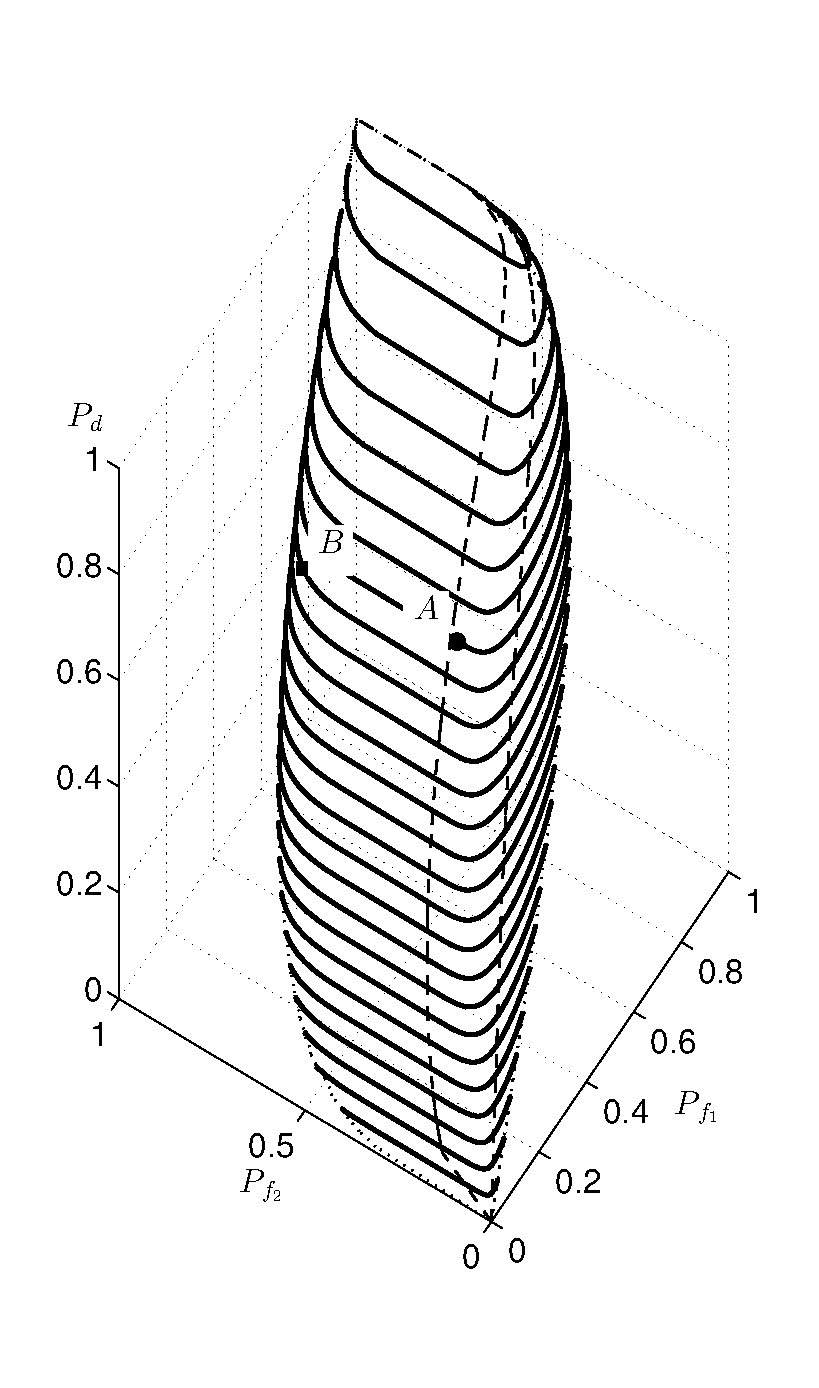
\includegraphics[width = 10cm, height=16cm]{2/ex1.eps}
\caption{The ROC surface for $k_1$, $k_2$ range from $-30$ to $30$ with step $0.01$.}
\label{fig: 2.1}
\end{figure}

\begin{figure}[!t]
\centering
\includegraphics[width = 10cm, height=16cm]{2/ex2.eps}
\caption{The ROC surface for problem \eqref{2015jan29a2}.}
\label{fig: 2.2mar9}
\end{figure}

\begin{figure}[!t]
\centering
\includegraphics[width = 10cm, height=16cm]{2/ex3.eps}
\caption{The contour for the ROC surface.}
\label{fig: 2.3mar9}
\end{figure}

Now let us consider points $A$ and $B$ on the ROC surface of Fig. \ref{fig: 2.1}, which are marked with '$\bullet$' and '$\blacklozenge$', respectively.  The coordinate of point $A$ is $(P_{f_1}, P_{f_2}, P_d) = (0.350, 0.315, 0.730)$; and the coordinate of point $B$ is  $(P_{f_1}, P_{f_2}, P_d) = (0.355, 0.730, 0.690)$. We can see even through $P_{f_1}$ and $P_{f_2}$ of point $B$ is larger than these of point $A$, the $P_d$ of point $B$ is  smaller than that of point $A$.  
Unlike NP test, where $P_d$ is always non-decreasing with $P_f$, in the case of multiple hypotheses testing (Extended Neyman Pearson Test), $P_d$ is not always a non-decreasing function of  $P_{f_i}$ ($i=1, ..., M$).

Furthermore, we can see in the case of point $B$, the value of $P_d$ is smaller than the value of $P_{f_2}$, i.e. under the ENP framework, $P_d \geq P_{f_i}$  ($i = 1, ..., M$) does not always hold (Qian Zhang arrives at the same conclusion in  \cite{zhang1999design, zhang2000efficient} using a different method). 

\subsection{Four Lemmas for the ENP Test}
Next we presents four lemmas concerning the properties of the ENP test.

%LEMMA 1
\newcommand{\bmu}{\boldsymbol{\mu}}
\typeout{}
\noindent \textbf{Lemma 1}
\noindent \textit{Let $f_0$, $f_1$, ..., $f_M$ be PDFs defined on set $\mathcal{D}$. For given constants $c_1, ..., c_M \in [0, 1]$, let $\mathcal{C}_\delta$ denote a set of decision rules,  such that for $\delta \in \mathcal{C}_\delta$, we have $P_{f_i} \leq c_i$, $i = 1, \cdots, M$. Then we have:
 among all members of $\mathcal{C}_\delta$ there exists one that maximizes $P_d$.}

\noindent \textbf{PROOF}
Define $\boldsymbol{\mu}_0^T = [\mu_1, ..., \mu_M]$  and  $\mathbf{P}_f^T = [P_{f_1}, P_{f_2}, ..., P_{f_M}]$ that are vectors in an $M$ dimensional Euclidean  space. Let $\bmu^T = [\bmu_0^T, \mu_{M+1}]$ denote a vector in $M+1$ dimensional Euclidean space. 
Let $P_d(\delta)$, $P_{f_i}(\delta)$ denote the $P_d$ and $P_{f_i}$ achieved by using decision rule $\delta$.
%By $\mathbf{A} \leq \mathbf{B}$, $\mathbf{A} = \mathbf{B}$ and  $\mathbf{A} \geq \mathbf{B}$ we mean that every element of $\mathbf{A}$ is no larger than, equal to and no smaller than its corresponding element of $\mathbf{B}$, respectively. 
%By $\mathbf{A} \neq 0$, we mean that every element of $\mathbf{A}$ is not equal to $0$. 

Let us define the set of points in $M+1$ dimensional Euclidean space
\begin{equation}
\begin{split}
\label{2015apr28a0}
  \mathcal{N} = \{(\mu_1, \mu_2, ..., \mu_{M+1}) &| \mu_i = \int_{\mathcal{S}}f_i(x)\mathrm{d}x \;\;i=1, ..., M,\\
                                            &  \mu_{M+1}=\int_{\mathcal{S}}f_{0}(x)\mathrm{d}x \;\;\text{ for an $\mathcal{S}$}\}
\end{split}
\end{equation}
We can see that $\mathcal{N}$ is the set of point $(\bmu_0, \mu_{M+1})=(\mathbf{P}_f(\delta), P_d(\delta))$, where $\delta$ is a decision rule. According to \cite{LehmannTest}, set $\mathcal{N}$ is a closed set. We consider one special point in set $\mathcal{N}$. When $\mathcal{S} = \emptyset$, we have $\mu_i = \int_{\emptyset}f_i(x)\mathrm{d}x = 0$, $i = 1, ..., M+1$, i.e. point $(\mu_1, ..., \mu_{M+1}) = (0, ..., 0)$ is an element of set $\mathcal{N}$.

Define the set of points in $M+1$ dimensional Euclidean Space 
\begin{equation}
\mathcal{P} = \{
(\mu_1, \mu_2, ..., \mu_{M+1}) | \bmu_0 \in [0^M, \mathbf{c}], \mu_{M+1} \in [0, 1]
\}\,.
\end{equation}
Clearly set $\mathcal{P}$ is a closed set and point $(\mu_1, ..., \mu_{M+1}) = (0, ..., 0)$ is an element  of set $\mathcal{P}$.


Let $\mathcal{K} = \mathcal{N} \cap \mathcal{P}$, hence we have
\begin{equation}
\label{apr14a0}
\mathcal{K} = \{
(\mu_1, \mu_2, ..., \mu_{M+1}) | (\bmu_0, \mu_{M+1}) \in \mathcal{N} \text{ and } \bmu_0 \in [0^M, \mathbf{c}], \mu_{M+1} \in [0, 1]
\}\,.
\end{equation}

Point $(\mu_1, ..., \mu_{M+1}) = (0, ..., 0)$ belongs to set $\mathcal{N}$ and set $\mathcal{P}$, hence it belongs to set $\mathcal{K}$. This suggests set $\mathcal{K}$ is not an empty set.
As both $\mathcal{N}$ and $\mathcal{K}$ are closed set, $\mathcal{K}$ is also closed \cite{rudin1964principles}. Besides that, for a point  $(\mu_1, \mu_2, ..., \mu_{M+1}) \in \mathcal{K}$, we have $\mu_i \in [0, c_i]$ and $\mu_{M+1} \in [0,1]$. Thus we can conclude set $\mathcal{K}$ is a bounded set. As $\mathcal{K}$ is a closed and bounded set in $M+1$ Euclidean Space, it is compact \cite{johnsonbaugh2012foundations}. 

Define function $f: \mathbf{R}^{M+1} \rightarrow \mathbf{R}$ as
\begin{equation}
f(\mu_1, \mu_2, ..., \mu_{M+1}) = \mu_{M+1}\,.
\end{equation}

It is easy to see $f$ is a continuous function. According to \cite{johnsonbaugh2012foundations}, $f$ attains a maximum and minimum value on set $\mathcal{K}$. 
Without losing generality, assume $f(\bmu^0)  = \mu_{M+1}^0$ (where $\bmu^0 = (\mu_1^0, \cdots, \mu_{M+1}^0)$ and $\bmu^0 \in \mathcal{K}$) achieve this maximum value. 
Since $\bmu^0 \in \mathcal{K}$ and $\mathcal{K}  \subseteq  \mathcal{N}$, from the definition of $\mathcal{N}$, there exists a decision rule $\delta^\ast$ such that $(\mathbf{P}_{f}(\delta^\ast), P_d(\delta^\ast)) = \bmu^0$.  
Furthermore, since $\bmu^0 \in \mathcal{K} $, from the definition of $\mathcal{K}$ we know $\mathbf{P}_{f}(\delta^\ast) \leq \mathbf{c}$, 
i.e. $\delta^\ast$ is a member of $\mathcal{C}_\delta$. 
Let $\delta' $ be a decision rule in set $\mathcal{C}_\delta$, 
from the definition of $\mathcal{C}_{\delta}$,   
it can be seen that $(\mathbf{P}_f(\delta'), P_d(\delta')) \in \mathcal{N}$ and $(\mathbf{P}_f(\delta'), P_d(\delta')) \in \mathcal{P}$, hence  $(\mathbf{P}_f(\delta'), P_d(\delta')) \in \mathcal{K}$.
Since $f(\bmu^0) = \mu_{M+1}^0$ achieves the maximum value for $\bmu \in \mathcal{K}$, we have
$f(\mathbf{P}_f(\delta'), P_d(\delta'))  = P_d(\delta') \leq  f(\bmu^0) = \mu_{M+1}^0 =  P_d(\delta^\ast)$. 
This suggests for a decision rule $\delta' \in \mathcal{C}_\delta$, we have $P_d(\delta^\ast) \geq P_d(\delta')$, i.e. $\delta^\ast$ maximize $P_d$ among all members of $\mathcal{C}_\delta$.

Q.E.D.


\noindent \textbf{Lemma 2}
\noindent \textit{
Let $f_0$, $f_1$, ..., $f_M$ be PDFs defined on set $\mathcal{D}$. For given constants $c_1, ..., c_M \in (0, 1)$, let $\mathcal{C}_\delta$ denote a set of decision rules,  such that for any $\delta \in \mathcal{C}_\delta$, we have $P_{f_i} \leq c_i$, $i = 1, \cdots, M$.
%No. 1
%\\\textnormal{(\rmnum{1})} Among all members of $\mathcal{C}_\mathcal{S}$ there exists one that maximizes $P_d$.
%No.2
If  $\delta^{\ast}$ is a member of $\mathcal{C}_\delta$ and it maximize $P_d$ among all members of $\mathcal{C}_\delta$, then there exists non-negative constants $k_1, ..., k_M$ such that $\delta^\ast$ can be written in form of  
\begin{equation}
f_0(x) \substack{H_0 \\ \geq \\ < \\ \bar{H}_0} \sum_{j=1}^{M}k_jf_j(x)
\end{equation}
Moreover, under decision rule $\delta^\ast$ if  $P_{f_i} < c_i$, then $k_i = 0$. 
}

In \cite{zhang1999design, zhang2000efficient} Qian Zhang also arrives at the conclusion that if $P_{f_i} < c_i$ then $k_i = 0$, through analysing the change of $P_d$ with respect to $k_i$ (he shows if $P_{f_i} < c_i$ and $k_i > 0$, then the $P_d$ can be further increased through adjusting the value of $k_i$). In the following we will prove \textbf{Lemma 1} using a mathematical method such that used in \cite{LehmannTest, dantzig1951fundamental} to prove the ENP Lemma (\rmnum{4}).

\noindent\textbf{PROOF}
We start by defining some notations for easy presentation.
Define $\mathbf{c}^T = [c_1, c_2, ..., c_M]$ and  $\mathbf{k}^T = [k_1, k_2, ..., k_M]$  are vectors in an $M$ dimensional Euclidean  space. Let $\bmu^T = [\bmu_0^T, \mu_{M+1}]$ denote a vector in $M+1$ dimensional Euclidean space. 

Let $F(\boldsymbol{\mu}_0)$ denote the largest $P_d$ under the constraints $P_{f_i} = \mu_i\;\;i = 1, ..., M$.
Let $G(\boldsymbol{\mu}_0)$ denote the largest $P_d$ under the constraints $P_{f_i} \leq \mu_i\;\;i = 1, ..., M$.
By $\mathbf{A} \leq \mathbf{B}$, $\mathbf{A} = \mathbf{B}$ and  $\mathbf{A} \geq \mathbf{B}$ we mean that every element of $\mathbf{A}$ is no larger than, equal to and no smaller than its corresponding element of $\mathbf{B}$, respectively. 
By $\mathbf{A} \neq 0$, we mean that every element of $\mathbf{A}$ is not equal to $0$. 
Let $G'$ denote the hyper surface in an $M+1$ dimensional Euclidean Space defined by 
\begin{equation}
 \label{def: G'}
 G' = \{(\bmu_0, \mu_{M+1})  | \bmu_0 \in [0, 1]^M, \mu_{M+1}= G(\bmu_0) \}\,.
\end{equation}
Let $G_s$ denote the set of points in an $M+1$ Euclidean space defined as 
\begin{equation}
  \label{2015feb16n1}
G_s =  \{(\boldsymbol{\mu}_0, \mu_{M+1}) | \boldsymbol{\mu}_0\in [0, 1]^M, \mu_{M+1} \in [0, G(\mathbf{\bmu_0})]
    \}\,.
  \end{equation}
  From \eqref{def: G'} and \eqref{2015feb16n1}, it can be seen $G' \in G_s$. Fig. \ref{fig: feb18} depicts the relationship between $G'$ and $G_s$ when $M=2$. In Fig. \ref{fig: feb18}, $G'$ is the surface enclosed by curve $\stackrel\frown{AC}$, curve $\stackrel\frown{AD}$, segment $\overline{OC}$ and segment $\overline{OD}$. Set $G_s$ is the space enclosed by plane $ABC$, plane $ABD$, plane $COD$ and surface $G'$.  

\begin{figure}[!t]
\centering
\includegraphics[width = 12cm, height=16cm]{2/example_pic.eps}
\caption{Relationship between $G'$ and $G_s$}
\label{fig: feb18}
\end{figure}
As we defined in \eqref{2015apr28a0}, $\mathcal{N}$ is the set of point $(\bmu_0, \mu_{M+1})=(\mathbf{P}_f(\delta), P_d(\delta))$, where $\delta$ is a decision rule.
From the definition of $\mathcal{N}$ and $F(\bmu_0)$ we can conclude that for a point $(\bmu_0, \mu_{M+1}) \in \mathcal{N}$, we have $\mu_{M+1} \leq F(\bmu_0)$. 
To see this, assume $\mu_{M+1} > F(\bmu_0)$. Then there is a decision rule $\delta$ such that $P_{f_i}(\delta) = \mu_i$ ($i=1, ..., M$) and $P_d(\delta) > F(\bmu_0)$. This is contradictory to the definition of $F(\bmu_0)$. 

The whole proof consists of the following parts: first we prove $G(\boldsymbol{\mu}_0)$ is a convex, non-decreasing function, and when $\boldsymbol{\mu}_0 > 0$, $G(\boldsymbol{\mu}_0) > 0$;
secondly it will be shown that $G_s$ is a convex set and $\mathcal{N} \subseteq G_s$; 
after that we will illustrate that for a point $(\mu_1^0, \mu_2^0, ..., \mu_{M+1}^0) \in G'$, there exists a non-negative $\mathbf{k}$ such that 
\[
\mu_{M+1} - \sum_{i=1}^{M}k_i\mu_i \leq \mu_{M+1}^0 - \sum_{i=1}^{M}k_i\mu_i^0
\]
holds for point $(\mu_1, \mu_2, ..., \mu_{M+1}) \in G_s$;
at the end, we will show for $\mathbf{c} \in (0, 1)$, there exists a non-negative $\mathbf{k}$ such that the optimal decision rule to achieve the largest $P_d$ under constraint $\mathbf{P}_f \leq \mathbf{c}$ can be written in the form
\[
f_0(x) \substack{H_0 \\ > \\ < \\ \bar{H}_0} \sum_{i=1}^{M}k_if_i(x)\,.
\]

Firstly we will prove $G(\bmu_0)$ is a convex non-decreasing function in each variable $\mu_i$, $i = 1, \cdots, M$.
 Let $\boldsymbol{\mu}^1$ and  $\boldsymbol{\mu}^2$ be two points on $G'$ with coordinates $(\boldsymbol{\mu}^1_0, \mu_{M+1}^1)$ and $(\boldsymbol{\mu}^2_0, \mu_{M+1}^2)$, i.e. $\mu_{M+1}^1 = G(\boldsymbol{\mu}_0^1)$ and $\mu_{M+1}^2 = G(\boldsymbol{\mu}_0^2)$. Let $\delta_1$ be a decision rule which can achieve the largest $P_d$ under the constraint $\mathbf{P}_f \leq \boldsymbol{\mu}_0^1$ and $\delta_2$ be a decision rule which can achieve the largest $P_d$ under the constraint $\mathbf{P}_{f} \leq \boldsymbol{\mu}_0^2$. Thus we can see 
 \begin{subequations}
\begin{align}
&\mu_{M+1}^1 = P_d(\delta^1) = G(\boldsymbol{\mu}_0^1)\\
&\mu_{M+1}^2 = P_d(\delta^2)=G(\boldsymbol{\mu}_0^1)\\
&\mathbf{P}_f(\delta^1) \leq \boldsymbol{\mu}^1_0\\
&\mathbf{P}_f(\delta^2) \leq \boldsymbol{\mu}^2_0
\end{align}
 \end{subequations}
 
Construct a new randomized test $\delta^3$, where $\delta^1$ and $\delta^2$ are used with equal probability. With decision rule $\delta^3$, we have 
\begin{subequations}
\begin{align}
\label{1120night1}
&P_d(\delta^3) = 0.5P_d(\delta^1)+0.5P_d(\delta^2) = 0.5G(\bmu_0^1) + 0.5G(\bmu_0^2)\\
&\mathbf{P}_{f}(\delta^3) = 0.5\mathbf{P}_f(\delta^1)+0.5\mathbf{P}_f(\delta^2) \leq 0.5\boldsymbol{\mu}^1_0 + 0.5\boldsymbol{\mu}^2_0
\end{align}
\end{subequations}
Let $\delta'$ denote the optimal decision rule for 
 \begin{equation}
 \begin{split}
 \label{1120t}
 \max&\;\;\;\;P_d\\
 \text{s.t.}&\;\;\;\;\mathbf{P}_f \leq 0.5\boldsymbol{\mu}^1_0 + 0.5\boldsymbol{\mu}^2_0
 \end{split}
 \end{equation}
then obviously $P_d(\delta') \geq P_d(\delta^3)$ (otherwise $\delta'$ cannot be the optimal decision rule for \eqref{1120t}). Since $P_d = G(0.5\boldsymbol{\mu}^1_0 + 0.5\boldsymbol{\mu}^2_0)$, we have  
\begin{equation}
\label{1120t2}
G(0.5\boldsymbol{\mu}^1_0 + 0.5\boldsymbol{\mu}^2_0) \geq  P_d(\delta^3).
\end{equation}
Substituting \eqref{1120night1} in \eqref{1120t2} results in
\begin{equation}
\label{1120t3}
G(0.5\boldsymbol{\mu}^1_0 + 0.5\boldsymbol{\mu}^2_0) \geq 0.5 G(\boldsymbol{\mu}^1_0)+ 0.5 G(\boldsymbol{\mu}^2_0)\,.
\end{equation}
showing that  $G(\bmu_0)$ is a convex function for $\bmu_0 \in [0, 1]^M$.

According to the definition of $G(\bmu_0)$, when $\mu_i$ increases, the false alarm constraints are relaxed, 
so the value of $G(\bmu_0)$ will either remain the same or increase. 
This suggests $G(\bmu_0)$ is a non-decreasing function of $\bmu_0$. 
This is not contradictory with the conclusion that 
$P_d$ is not always increasing with $P_{f_i}\;\;(i=1, 2, \cdots, M)$  (we arrived at this conclusion in Chapter 2 section 1.1 on page 12).  This is because $\bmu_0$ is not the probability of false alarms but rather the constraints of the probability of false alarm. 

Next we will show when $\boldsymbol{\mu}_0 > 0^M$, then $G(\boldsymbol{\mu}_0)$ is strictly larger than zero.
Let $\delta^\ast$ be the optimal decision rule for $\bmu_0$. By optimal  we mean that this decision rule provides the largest $P_d$ under the constraints $\mathbf{P}_f \leq \bmu_0$, i.e. $P_d(\delta^\ast) = G(\bmu_0)$. Consider two decision rule $\delta^1$ and $\delta^2$ defined as 
\begin{equation}
  \label{2015feb09a4}
  \delta^1:\;\; \begin{cases}
    & \;\;\;\text{ $H_0$ if } x \in \emptyset \\
    & \;\;\;\text{ $\bar{H}_0$ if } x \in \mathcal{D}
  \end{cases}
\end{equation}
and
\begin{equation}
  \label{2015feb09a5}
  \delta^2:\;\; \begin{cases}
    &x \;\;\;\text{ $H_0$ if } x \in \mathcal{D} \\
    &x \;\;\;\text{ $\bar{H}_0$ if } x \in \emptyset
  \end{cases}
\end{equation}

From \eqref{2015feb09a4} and \eqref{2015feb09a5} we can see the $P_d$ and $P_{f_i}$ under under decision rule $\delta^1$ and $\delta^2$ can be written as
\begin{equation}
  P_d(\delta^1) = \int_{\emptyset}f_0(x)\mathrm{d}x = 0
\end{equation}
\begin{equation}
    P_{f_i}(\delta^1) = \int_{\emptyset}f_i(x)\mathrm{d}x = 0
\end{equation}
\begin{equation}
    P_d(\delta^2) = \int_{\mathcal{D}}f_0(x)\mathrm{d}x = 1
\end{equation}
\begin{equation}
    P_{f_i}(\delta^2) = \int_{\mathcal{D}}f_i(x)\mathrm{d}x = 1
\end{equation}

Let $\mu_{min} = \min(\mu_1, \mu_2, \cdots, \mu_M)$. Since $\bmu_0 > 0^M$, we know $\mu_i > 0$ for $i = 1, \cdots, M$. Then we have $\min(\mu_1, \cdots, \mu_M) > 0$, i.e. $\mu_{min} > 0$. Construct a new randomized test $\delta^3$ where $\delta^1$ and $\delta^2$ are used with probability $1 - \mu_{min} $ and $\mu_{min}$. With decision rule $\delta^3$ we have
\begin{equation}
  P_d(\delta^3) = (1 - \mu_{min})P_d(\delta^1) + \mu_{min}P_d(\delta^2) = \mu_{min} > 0
\end{equation}
\begin{equation}
  P_{f_i}(\delta^3) = (1 - \mu_{min})P_{f_i}(\delta^1) + \mu_{min}P_{f_i}(\delta^2) = \mu_{min} \leq \mu_i \;\;\;\;(i = 1, 2, \cdots, M)
\end{equation}

Hence we can see by using $\delta^3$ we have
\[
  \mathbf{P}_f(\delta^3) \leq \bmu_0\,.
\]
Since $\delta^\ast $ is the optimal decision rule for $\bmu_0$, we can conclude $P_d(\delta^\ast) \geq  P_d(\delta^3) = \mu_{min} >  0$. Since $G(\bmu_0) = P_d(\delta^\ast)$, we can conclude $G(\bmu_0) > 0$ when $\bmu_0 > 0 $. 


In the following, we consider the property of $G_s$. First we will prove that $G_s$ is a convex set. 
Let $\boldsymbol{\mu}^1$ and  $\boldsymbol{\mu}^2$ be two points that belong to $G_s$ with coordinates $(\boldsymbol{\mu}^1_0, \mu_{M+1}^1)$ and $(\boldsymbol{\mu}^2_0, \mu_{M+1}^2)$. According to the definition of $G_s$, we have 
\begin{subequations}
\label{1120t4}
\begin{align}
\label{1120night6}
&0^M \leq \bmu_0^1 \leq 1^M\\
\label{1120night7}
&0^M \leq \boldsymbol{\mu}^2_0 \leq 1^M\\
\label{1120night3}
&0 \leq \mu_{M+1}^1 \leq G(\boldsymbol{\mu}_0^1)\\
\label{1120night4}
&0 \leq \mu_{M+1}^2 \leq G(\boldsymbol{\mu}_0^2)
\end{align}
\end{subequations}

Let $\boldsymbol{\mu}^3$ be the middle point between $\boldsymbol{\mu}^1$ and $\boldsymbol{\mu}^2$ with coordinate $(\bmu_0^3, \mu_{M+1}^3)$, where  
\begin{subequations}
\label{1120t5}
\begin{align}
\label{1120night5}
\bmu_0^3 &= 0.5\boldsymbol{\mu}_0^1 + 0.5 \boldsymbol{\mu}_0^2\\
\label{1120night2}
\mu_{M+1}^3 &= 0.5 \mu_{M+1}^1 + 0.5 \mu_{M+1}^2
\end{align}
\end{subequations}
In the following, we will show $\bmu^3 \in G_s$.  
From \eqref{1120night6}, \eqref{1120night7} and \eqref{1120night5} we can see that
\begin{equation}
\label{equ: 1120n1}
\bmu_0^3 \in [0, 1]^M
\end{equation}
Substituting \eqref{1120night3} \eqref{1120night4} into \eqref{1120night2}, we have
\begin{equation}
  \label{equ:2015feb1a}
0 \leq \mu_{M+1}^3 \leq 0.5 G( \bmu_0^1) + 0.5G(\bmu_0^2)\,.
\end{equation} 
Using \eqref{1120t3} and \eqref{1120night5} with \eqref{equ:2015feb1a} gives,
\begin{equation}
\label{equ: 1120n}
0 \leq \mu_{M+1}^3 \leq G(0.5 \bmu_0^1 + 0.5\bmu_0^2) = G(\bmu_0^3)\,.
\end{equation}
From \eqref{equ: 1120n} and \eqref{equ: 1120n1}, it follows that  
 $\bmu^3 \in G_s$, showing that $G_s$  is a convex set.  

Next we prove $\mathcal{N} \subseteq G_s$. We need to show that if  $\forall (\mu_1, ..., \mu_{M+1}) \in \mathcal{N}$, then this point also belongs to $G_s$.
Assume $(\mu_1^N, ..., \mu_{M+1}^N)$ is a point in $\mathcal{N}$. 
In previous discussion, it has been shown $\mu_i^N \in [0, 1]$ ($i = 1, ..., M$) and $\mu_{M+1}^N \in [0, F(\bmu_0^N)]$, where $\bmu_0^N = [\mu_1^N, ..., \mu_M^N]$. 
According to the definition of $G(\bmu_0)$ and $F(\bmu_0)$, we can conclude $G(\bmu_0^N) \geq F(\bmu_0^N)$. 
This implies $\mu_{M+1}^N \in [0, G(\bmu_0^N)]$ and we have  
\begin{equation}
\begin{split}
&\mu_i^N \in [0, 1]\;\;\;\;(i=1, 2, ..., M)\\
&\mu_{M+1}^N \in [0, G(\bmu_0^N)]
\end{split}
\end{equation}
showing that point $(\mu_1^N, ..., \mu_{M+1}^N)$ also belongs to set $G_s$.
Hence we proved $\mathcal{N} \subseteq G_s$. 

In the following we will show for any point $(\mu_1^0, \mu_2^0, ..., \mu_{M+1}^0)$ that belongs to $G'$ ($\mu_i^0 \in (0, 1), i = 1, 2, ..., M$), there exists a non-negative $\mathbf{k}$ such that  
\[
\mu_{M+1} - \sum_{i=1}^{M}k_i\mu_i \leq \mu_{M+1}^0 - \sum_{i=1}^{M}k_i\mu_i^0
\]
holds for any $(\mu_1, \mu_2, ..., \mu_{M+1}) \in G_s$. 
Assume $(\mu_0^0, \mu_1^0, ..., \mu_{M+1}^0)$ is a point on the $G'$ surface, i.e. $\mu_{M+1}^0 = G(\bmu_0^0)$, where $\bmu_0^0 = [\mu_1^0, ..., \mu_{M}^0]$. 
Also we assume $\mu_1^0, \mu_2^0, ..., \mu_M^0 \in (0, 1)$. 
According to the definition of $G_s$, for any positive $\epsilon$, point $(\mu_0^0, \mu_1^0, ..., \mu_{M+1}^0+\epsilon) \notin G_s$. Thus point $(\mu_1^0, ..., \mu_{M+1}^0)$ is a boundary point of the set $G_s$.  
Since $G_s$ is a convex set and $(\mu_0^0, \mu_1^0, ..., \mu_{M+1}^0)$ is a boundary point of $G_s$,  
there exists an $M+1$-dimensional hyperplane $\Pi$ through this point such that $\Pi$ contains only boundary points of $G_s$ and $G_s$ lies entirely on one sides of $\Pi$  \cite{dantzig1951fundamental}. 
There exists $k_i^0$ ($i=1, ..., M+1$) such that the equation defining $\Pi$ can be written as \cite{dantzig1951fundamental}
\begin{equation}
\label{PI}
k_{M+1}^0\mu_{M+1} - \sum_{i=1}^{M}k_i^0\mu_i = k_{M+1}^0\mu_{M+1}^0 - \sum_{i=1}^{M}k_i^0\mu_i^0
\end{equation}

In section 2.2.2, we have proved that when $\mu^0_i\neq 0$ ($i=1, ..., M$), $\mu_{M+1}^0 = G(\bmu_0^0) $ is strictly larger than zero, i.e. $\mu_{M+1}^0 > 0$. Hence there exists a $\mu_{M+1}' = \frac{\mu_{M+1}^0}{2}$ such that $\mu_{M+1}' \in (0, \mu_{M+1}^0)$. From the definition of $G_s$, it is easy to see that point $(\mu^0_1, ..., \mu^0_M, \mu_{M+1}')$ also belongs to set $G_s$. Besides that, since $\mu^0_i \in (0, 1)$ ($i=1, ..., M$) and $\mu_{M+1}' \in (0, \mu_{M+1}^0)$, it can be concluded that point $(\mu_1^0, \mu_2^0, ..., \mu_{M+1}')$ is an inner point of $G_s$.
From previous discussion about hyperplane $\Pi$, we can see that point $(\mu^0_1, ..., \mu^0_M, \mu_{M+1}')$ is not contained in hyperplane $\Pi$, i.e.
\[
k_{M+1}^0\mu_{M+1}' - \sum_{i=1}^{M}k_i^0\mu_i^0 \neq k_{M+1}^0\mu_{M+1}^0 - \sum_{i=1}^{M}k_i^0\mu_i^0
\]
\[
\therefore k_{M+1}^0\mu_{M+1}' \neq k_{M+1}^0\mu_{M+1}^0
\]
\[
\therefore k_{M+1}^0 \neq 0
\]
With $k_i = \frac{k_i^0}{k_{M+1}^0}$, the equation defining the hyperplane $\Pi$ can be written as
\begin{equation}
\label{PI2}
\mu_{M+1} - \sum_{i=1}^{M}k_i\mu_i = \mu_{M+1}^0 - \sum_{i=1}^{M}k_i\mu_i^0\,,
\end{equation}
on equivalently 
\begin{equation}
\label{PI2b}
\mu_{M+1} - \sum_{i=1}^{M}k_i\mu_i - (\mu_{M+1}^0 - \sum_{i=1}^{M}k_i\mu_i^0) = 0\,.
\end{equation}

From \cite{planeside} we have that $\Pi$ divides the space into two parts, on one side of $\Pi$ consisting of  points that satisfy
\begin{equation}
\mu_{M+1} - \sum_{i=1}^{M}k_i\mu_i - (\mu_{M+1}^0 - \sum_{i=1}^{M}k_i\mu_i^0) > 0\,;
\label{2014apr25a2}
\end{equation}
and the other part on the other side of $\Pi$ consisting of points that satisfy
\begin{equation}
\mu_{M+1} - \sum_{i=1}^{M}k_i\mu_i - (\mu_{M+1}^0 - \sum_{i=1}^{M}k_i\mu_i^0) < 0\,.
\label{2015apr25a3}
\end{equation}

Since point $(\mu_1^0, ..., \mu_M^0, \mu_{M+1}')$ is not contained in hyperplane $\Pi$, it either satisfies \eqref{2014apr25a2} or \eqref{2015apr25a3}. From the condition that $\mu_{M+1}' = \frac{\mu_{M+1}^0}{2}$ and $\mu_{M+1}^0 > 0$, we can see point  $(\mu_1^0, ..., \mu_M^0, \mu_{M+1}')$ satisfies \eqref{2015apr25a3}.  
Furthermore, since $\mu_i^0 \in (0, 1)$, from the definition of $G_s$, we can see that point $(\mu_1^0, ..., \mu_M^0, \mu_{M+1}')$ belongs to set $G_s$. 
Since point $(\mu_1^0, ..., \mu_M^0, \mu_{M+1}')$ satisfies \eqref{2015apr25a3} and since $G_s$ lies entirely on one side of hyper plane $\Pi$, to make all points belonging to $G_s$ lies on the same side of $\Pi$ as point $(\mu_1^0, ..., \mu_M^0, \mu_{M+1}')$ does, we must have
%Since $G_s$ lies entirely on one side of \eqref{PI2}, and since when $(\mu_1, ... ,\mu_M, \mu_{M+1})=(\mu_1^0, ..., \mu_M^0, 0)$, the left-hand of \eqref{PI2} is smaller than the right-hand, we must have 
\begin{equation}
\mu_{M+1} - \sum_{i=1}^{M}k_i\mu_i -  ( \mu_{M+1}^0 - \sum_{i=1}^{M}k_i\mu_i^0) \leq 0
\label{PI3}
\end{equation}
on equivalently,
\[
\mu_{M+1} - \sum_{i=1}^{M}k_i\mu_i \leq   \mu_{M+1}^0 - \sum_{i=1}^{M}k_i\mu_i^0
\]
for all the points belong to $G_s$ \cite{dantzig1951fundamental, planeside}. 

Up to now, we have proved that if  $(\bmu_0^0, \mu_{M+1}^0) \in G'$ and $\bmu_0^0 \in (0, 1)^M$, there exists constants $k_1$, ..., $k_M$ such that
\begin{equation}
\mu_{M+1} - \sum_{i=1}^{M}k_i\mu_i \leq \mu_{M+1}^0 - \sum_{i=1}^{M}k_i\mu_i^0
\label{PPI3}
\end{equation}
holds for  $(\mu_1, \mu_2, ...\mu_{M+1}) \in G_s$. 
\eqref{PPI3} suggests that for a point on the hyper surface $G'$ with coordinate $(\bmu_0^0, \mu_{M+1}^0)$, where $\bmu_0^0 \in (0, 1)$, then there exists a hyper  plane $\Pi$ 
\[
\mu_{M+1} - \sum_{i=1}^{M}k_i\mu_i =  \mu_{M+1}^0 - \sum_{i=1}^{M}k_i\mu_i^0 
\]
such that $G_s$ lies entirely on one side of $\Pi$. 

In the following, we will show that the constants $k_i$ in \eqref{PPI3} must be non-negative.   

Now consider another point on $G'$ with coordinate $(\mu_1^0, ..., \mu_l^0+\epsilon, ..., \mu_M^0, \mu_{M+1}'')$, where $\epsilon > 0$ and $l$ is an integer between $1$ and $M$.  Since both points $(\mu_1^0, ..., \mu_l^0, ..., \mu_M^0, \mu_{M+1}^0)$ and $(\mu_1^0, ..., \mu_l^0+\epsilon, ..., \mu_M^0, \mu_{M+1}'')$ lies on $G'$, we can conclude $G([\mu_1^0, ..., \mu_l^0, ...., \mu_M^0]) = \mu_{M+1}^0$ and $G([\mu_1^0, ..., \mu_l^0 + \epsilon, ...., \mu_M^0]) = \mu_{M+1}''$. As we proved $G(\bmu_0)$ is a non-decreasing function, we must have  $\mu_{M+1}'' \geq \mu_{M+1}^0$.
Substituting $(\mu_1^0, ..., \mu_l^0+\epsilon, ..., \mu_M^0, \mu_{M+1}'')$ into the left side of \eqref{PPI3}, we have
\begin{equation}
\mu_{M+1}'' - k_1\mu_1^0 - ... - k_l(\mu_l^0+\epsilon)- ... - k_M\mu_M^0 \leq \mu_{M+1}^0 - k_1\mu_1^0 - ... - k_l\mu_l^0- ... - k_M\mu_M^0
\end{equation}
\begin{equation}
\therefore \mu_{M+1}'' - k_l(\mu_l^0+\epsilon)\leq \mu_{M+1}^0 - k_l\mu_l^0
\end{equation}
\begin{equation}
\mu_{M+1}'' - \mu_{M+1}^0 \leq k_l\epsilon
\end{equation}
\begin{equation}
\therefore k_l \geq \frac{\mu_{M+1}'' - \mu_{M+1}^0}{\epsilon} \geq 0 \;\;\;\;l = 1, 2, \cdots, M
\label{2015feb16a1}
\end{equation}
From \eqref{2015feb16a1} we can see that the constants $k_l$ ($l = 1, 2, \cdots, M$) in \eqref{PPI3} are non-negative.
As we have proved if  $(\bmu_0^0, \mu_{M+1}^0) \in G'$ and $\bmu_0^0 \in (0, 1)^M$, there exists constants $k_1, ..., k_M$ such that  
\begin{equation}
\mu_{M+1} - \sum_{i=1}^{M}k_i\mu_i \leq \mu_{M+1}^0 - \sum_{i=1}^{M}k_i\mu_i^0
\label{PPI32015bc}
\end{equation}
holds for  $(\mu_1, \mu_2, ...\mu_{M+1}) \in G_s$ and the constants $k_1, k_2, \cdots, k_M$ are non-negative,  
we can conclude 
if  $(\bmu_0^0, \mu_{M+1}^0) \in G'$ and $\bmu_0^0 \in (0, 1)^M$, there exists constants $k_1, ..., k_M \geq 0 $ such that  
\eqref{PPI32015bc}
holds for  $(\mu_1, \mu_2, ...\mu_{M+1}) \in G_s$. 

For the given constants $\mathbf{c}$ ($\mathbf{c} \in (0, 1)^M$), 
 assume a decision rule $\delta^\ast$  achieves the largest $P_d$  while keeping $\mathbf{P}_f \leq \mathbf{c}$. In the following we will prove there exists non-negative $\mathbf{k}$  such that $\delta^\ast$ can be written in form of 
\[
f_0(x) \substack{H_0 \\ > \\ < \\ \bar{H}_0 } \sum_{i=1}^{M}k_if_i(x)\,.
\]

Let $\bmu_0 = \mathbf{c}$. According to the definition of $G'$, we can see that $(\mathbf{c},G(\mathbf{c})) \in G'$.  As $\delta^\ast $ achieves the largest $P_d$ under constraint $\mathbf{P}_f \leq \mathbf{c}$, from the definition of $G(\bmu_0)$ we can see $P_{d}(\delta^\ast) = G(\mathbf{c})$. 
Since we have proved if $(\bmu_0^0, \mu_{M+1}^0) \in G'$ and $\bmu_0^0 \in (0, 1)^M$, there exists non-negative constants $k_1$, ..., $k_M$ such that
\begin{equation}
\mu_{M+1} - \sum_{i=1}^{M}k_i\mu_i \leq \mu_{M+1}^0 - \sum_{i=1}^{M}k_i\mu_i^0
\label{PPI32015}
\end{equation}
holds for all points belonging $G_s$ and $(\mathbf{c},G(\mathbf{c})) \in G'$, we can see there exists non-negative $\mathbf{k}$ such that  

%According to the definition of $G(\bmu_0)$, we can see $P_d(\delta^\ast) = G(\mathbf{c})$. Since $(\mathbf{c}, G(\mathbf{c}))$is a point on the hyper surface $G'$,  there exists non-negative $\mathbf{k}$ such that 
\begin{equation}
\label{TEMP}
\mu_{M+1} - \sum_{i=1}^{M}k_i\mu_i \leq G(\mathbf{c}) - \sum_{i=1}^{M}k_ic_i
\end{equation}
holds for $(\mu_1, \mu_2, ..., \mu_{M+1}) \in G_s$.
Since $P_{f_i}(\delta^\ast) \leq c_i$ (for $i=1, ..., M$) and $k_i \geq 0$, we have  
\[
k_ic_i \geq k_iP_{f_i}(\delta^\ast)
\]
\[
\therefore \sum_{i=1}^{M}k_ic_i \geq \sum_{i=1}^{M}k_iP_{f_i}(\delta^\ast)
\]
Hence 
\begin{equation}
\label{con: 1}
G(\mathbf{c}) - \sum_{i=1}^{M}k_ic_i \leq G(\mathbf{c}) - \sum_{i=1}^{M}k_iP_{f_i}(\delta^\ast)\,.
\end{equation}
From \eqref{TEMP} and \eqref{con: 1}, we have 
\begin{equation}
\label{equ: TEMP3}
\mu_{M+1} - \sum_{i=1}^{M}k_i\mu_i \leq G(\mathbf{c}) - \sum_{i=1}^{M}k_ic_i \leq G(\mathbf{c}) - \sum_{i=1}^{M}k_iP_{f_i}(\delta^\ast)
\end{equation}
\begin{equation}
\label{ASD}
\therefore \mu_{M+1} - \sum_{i=1}^{M}k_i\mu_i \leq G(\mathbf{c}) - \sum_{i=1}^{M}k_iP_{f_i}(\delta^\ast)
\end{equation}
Substitute $G(\mathbf{c}) = P_d(\delta^\ast)$ into \eqref{ASD}, 
\begin{equation}
\label{TEMP2}
\mu_{M+1} - \sum_{i=1}^{M}k_i\mu_i \leq P_d(\delta^\ast) - \sum_{i=1}^{M}k_iP_{f_i}(\delta^\ast)\,,
\end{equation}
where $(\mu_0, ..., \mu_{M+1}) \in G_s$.

Since $\mathcal{N} \subseteq G_s$, \eqref{TEMP2} also holds for a point belonging to $\mathcal{N}$.
According to the definition of $\mathcal{N}$, for $(\mu_1, \mu_2, ..., \mu_{M+1} \in \mathcal{N})$, we have  
\begin{equation}
\label{def: mu}
\begin{cases}
\mu_i = \int_{\mathcal{S}}f_i(x)\mathrm{d}x \;\;\;\;i = 1, ..., M\\
\mu_{M+1} = \int_{\mathcal{S}}f_{0}(x)\mathrm{d}x
\end{cases}
\end{equation}
where $\mathcal{S}$ can be any subset of the domain $\mathcal{D}$. 

Since $P_{f_i}(\delta^\ast)$ and $P_{d}(\delta^\ast)$ can be written as
\begin{equation}
\label{def: pfd}
\begin{cases}
P_{f_i}(\delta^\ast) = \int_{\mathcal{S}^\ast}f_i(x)\mathrm{d}x\;\;\;\;i=1, ..., M\\
P_d(\delta^\ast) = \int_{\mathcal{S}^\ast}f_0(x)\mathrm{d}x
\end{cases}
\end{equation}
by substituting \eqref{def: mu} and \eqref{def: pfd} into \eqref{TEMP2}, we have: 
\[
\int_{\mathcal{S}}f_{0}(x)\mathrm{d}x - \sum_{i=1}^{M}k_i\int_{\mathcal{S}}f_i(x)\mathrm{d}x \leq \int_{\mathcal{S}^\ast}f_{0}(x)\mathrm{d}x - \sum_{i=1}^{M}k_i\int_{\mathcal{S}^\ast}f_i(x)\mathrm{d}x
\]
\[
\therefore 
\int_{\mathcal{S}}f_{0}(x)\mathrm{d}x - \sum_{i=1}^{M}\int_{\mathcal{S}}k_if_i(x)\mathrm{d}x \leq \int_{\mathcal{S}^\ast}f_{0}(x)\mathrm{d}x - \sum_{i=1}^{M}\int_{\mathcal{S}^\ast}k_if_i(x)\mathrm{d}x
\]
\begin{equation}
\label{TEMP4}
\therefore \int_{\mathcal{S}}(f_{0}(x)- \sum_{i=1}^{M}k_if_{i}(x))\mathrm{d}x \leq \int_{\mathcal{S}^\ast}(f_{0}(x)- \sum_{i=1}^{M}k_if_{i}(x))\mathrm{d}x 
\end{equation}
The integrand of the left  and right sides of \eqref{TEMP4} are the same. Hence to have  \eqref{TEMP4} hold for all set $\mathcal{S}$,  
then  $\mathcal{S}^\ast$ must  maximize 
\begin{equation}
\int_{\mathcal{S}}(f_{0}(x)\mathrm{d}x - \sum_{i=1}^{M}k_if_i(x))\mathrm{d}x
  \label{2015feb2a3}
\end{equation}
among all $\mathcal{S}$. To maximize \eqref{2015feb2a3}, $\mathcal{S}^\ast$ should include all the domain that $f_{0}(x)- \sum_{i=1}^{M}k_if_{i}(x) > 0$ and exclude the domain that $f_{0}(x)- \sum_{i=1}^{M}k_if_{i}(x) < 0$, i.e.   
 $\mathcal{S}^\ast$ satisfies
\[
x \in \mathcal{S}^\ast\;\;\;\;\text{if}\;\;\;\;f_{0}(x)- \sum_{i=1}^{M}k_if_{i}(x) > 0
\]
\[
x \notin \mathcal{S}^\ast\;\;\;\;\text{if}\;\;\;\;f_{0}(x)- \sum_{i=1}^{M}k_if_{i}(x) < 0
\]

Hence we can conclude that for a given vector of constraints for $\mathbf{P}_f$, denoted as $\mathbf{c} \in (0, 1)^M$, there exists a set of non-negative $\mathbf{k}$ such that 
the optimal decision rule can be written as 
\[
f_0(x) \substack{H_0 \\ > \\ < \\ \bar{H}_0 } \sum_{i=1}^{M}k_if_i(x)\,.
\]

Moreover, since \eqref{TEMP} holds for any point $(\mu_1, \mu_2, ..., \mu_{M+1}) \in \mathcal{N}$ and $(\mathbf{P}_f(\delta^\ast), P_d(\delta^\ast)) \in \mathcal{N}$, we can conclude 
\begin{equation}
P_d(\delta^\ast) - \sum_{i=1}^{M}k_iP_{f_i}(\delta^\ast) \leq G(\mathbf{c}) - \sum_{i=1}^{M}k_ic_i
\label{20150422a0}
\end{equation}
As we have shown $G(\mathbf{c}) = P_d(\delta^\ast)$, the \eqref{20150422a0} can be written as
\begin{equation}
 G(\mathbf{c}) - \sum_{i=1}^{M}k_ic_i \geq G(\mathbf{c}) - \sum_{i=1}^{M}k_iP_{f_i}(\delta^\ast)
\label{TEMP5}
\end{equation}
From \eqref{con: 1} and \eqref{TEMP5}  we can conclude
\[
G(\mathbf{c}) - \sum_{i=1}^{M}k_iP_{f_i}(\delta^\ast) =  G(\mathbf{c}) - \sum_{i=1}^{M}k_ic_i
\]
\[
\therefore  \sum_{i=1}^{M}k_iP_{f_i}(\delta^\ast) =  \sum_{i=1}^{M}k_ic_i
\]
Since $k_iP_{f_i}(\delta^\ast) \leq k_ic_i$ (for $i=1, ..., M$), the above equation can be fulfilled only if $k_iP_{f_i}(\delta^\ast) = k_ic_i$ (for $i=1, ..., M$). When for a certain $i$, if $P_{f_i}(\delta^\ast) < c_i$, then $k_i$ must be zero.

Q.E.D.

Upon examination  the optimal decision rule for a given probability of false alarm constraints, in the following we consider properties of the ROC surface, embodied by two lemmas with proof.  

\noindent \textbf{Condition 1}
\textit{
\noindent Let $f_i(x) \;\;i=0, 1, ..., M$ be the PDF induced by hypothesis $H_i$, and define $g(x) = f_0(x) - \sum_{j=1}^{M} k_jf_j(x)$ where $k_i$  ($i = 1, 2, ..., M$) are real numbers. Let $\mathcal{D} \in \mathbb{R}$ be an open set such that $\int_{\bar{\mathcal{D}}}f_i(x)=0\;\;i = 1, 2, ..., M$. Furthermore,  if $x_0$ is a solution  for $g(x) = 0 \;\;(x \in \mathcal{D})$, then there exists an integer $n$ such that  the $n$-th order derivative of $g(x_0)$ is not equal to zero $(g^{(n)}(x_0) \neq 0)$.
}

\noindent \textbf{Lemma 3}
\textit{
\noindent Under}
\textbf{Condition 1}
\textit{, let $\mathbf{P}$ be a point with coordinate $(P_d, P_{f_1}, ..., P_{f_M})$ on the ROC surface of the EPN test. If there exists a tangent hyperplane at $\mathbf{P}$, then its normal is parallel to the vector $\mathbf{n} = (-1, k_1, ..., k_M)$, where $k_i$ are the parameters of the ENP test achieving $\mathbf{P}$.
}

\noindent\textbf{PROOF}
Define $\mathbf{k} = [k_1, k_2, ..., k_M]^T$ and $\mathbf{P}_f = [P_{f_1}, P_{f_2}, ..., P_{f_M}]^T$. Since both $P_d$ and $\mathbf{P}_f$ are functions of $\mathbf{k}$, $\mathbf{P}_f(\mathbf{k}_0)$ denotes the value of $\mathbf{P}_f$ when $\mathbf{k} = \mathbf{k}_0$ and $P_d(\mathbf{k}_0)$ denotes the value of $P_d$ when $\mathbf{k} = \mathbf{k}_0$. Using Taylor's expansion \cite{zill2011advanced} for $\mathbf{P}_f$ and $P_d$,
\begin{equation}
\label{pro: pd}
P_d = P_d(\mathbf{k}_0) + \frac{\mathrm{d}P_d}{\mathrm{d}\mathbf{k}^T}\bigg{|}_{\mathbf{k}=\mathbf{k_0}}(\mathbf{k} - \mathbf{k}_0)
+ o(\mathbf{k} - \mathbf{k}_0)
\end{equation}

\begin{equation}
\label{pro: pf}
\mathbf{P}_f = \mathbf{P}_f(\mathbf{k}_0) + \frac{\mathrm{d}\mathbf{P}_f}{\mathrm{d}\mathbf{k}^T}\bigg{|}_{\mathbf{k}=\mathbf{k_0}}(\mathbf{k} - \mathbf{k}_0)
+ o(\mathbf{k} - \mathbf{k}_0)
\end{equation}
here $\mathbf{k} \rightarrow \mathbf{k}_0$.

Consider the hyperplane $y$ as a function of $\mathbf{x}$ defined by
\begin{equation}
\label{pro: y}
y = P_d(\mathbf{k}_0) + \frac{\mathrm{d}P_d}{\mathrm{d}\mathbf{k}^T}\bigg{|}_{\mathbf{k}=\mathbf{k_0}}(\mathbf{z} - \mathbf{k}_0)
\end{equation}
\begin{equation}
\label{pro: x}
\mathbf{x} = \mathbf{P}_f(\mathbf{k}_0) + \frac{\mathrm{d}\mathbf{P}_f}{\mathrm{d}\mathbf{k}^T}\bigg{|}_{\mathbf{k}=\mathbf{k_0}}(\mathbf{z} - \mathbf{k}_0)
\end{equation}
The above equations construct a tangent hyperplane for the ROC surface at point $(P_d(\mathbf{k}_0), \mathbf{P}_f^T(\mathbf{k}_0))$. Combining both equations  we get

\begin{equation}
\label{pro : y2}
y = P_d(\mathbf{k}_0) + \frac{\mathrm{d}P_d}{\mathrm{d}\mathbf{k}^T}\bigg{|}_{\mathbf{k}=\mathbf{k_0}}(
\frac{\mathrm{d}\mathbf{P}_f}{\mathrm{d}\mathbf{k}^T}\bigg{|}_{\mathbf{k}=\mathbf{k_0}}
)^{-1} (\mathbf{x} - \mathbf{P}_f(\mathbf{k}_0))
\end{equation}
Hence the normal for point $(P_d(\mathbf{k}_0), \mathbf{P}_f^T(\mathbf{k}_0))$ on ROC surface can be written as
\begin{equation}
\label{vec: normal}
[-1, \frac{\mathrm{d}P_d}{\mathrm{d}\mathbf{k}^T}\bigg{|}_{\mathbf{k}=\mathbf{k_0}}(
\frac{\mathrm{d}\mathbf{P}_f}{\mathrm{d}\mathbf{k}^T}\bigg{|}_{\mathbf{k}=\mathbf{k_0}}
)^{-1}
].
\end{equation}

In the following, we will prove $ \frac{\mathrm{d}P_d}{\mathrm{d}\mathbf{k}^T}(
\frac{\mathrm{d}\mathbf{P}_f}{\mathrm{d}\mathbf{k}^T}
)^{-1} = \mathbf{k}^T
$, which can be written as
\begin{equation}
\label{pro: vec}
\frac{\mathrm{d}P_d}{\mathrm{d}\mathbf{k}^T} = \mathbf{k}^T \frac{\mathrm{d}\mathbf{P}_f}{\mathrm{d}\mathbf{k}^T}
\end{equation}
which in component form can be written as 
\begin{equation}
\label{pro: component}
\frac{\partial P_d}{\partial k_i} - \sum_{n=1}^{M}k_n\frac{\partial P_{f_n}}{\partial k_i} = 0 \;\;\;\;(i=1, 2, ..., M).
\end{equation}
Using \eqref{equ: pf and pd} and calculating the  partial derivatives results in
\begin{equation}
\label{pro: Pf par k}
\frac{\partial P_{f_n}}{ \partial k_i} = - \int_{\mathcal{D}}\delta (f_0(x) - \sum_{j=1}^{M}k_jf_j(x))f_i(x)f_n(x) \mathrm{d}x\,,
\end{equation}
\label{pro: Pd par k}
\begin{equation}\frac{\partial P_d}{ \partial k_i} = - \int_{\mathcal{D}}\delta (f_0(x) - \sum_{j=1}^{M}k_jf_j(x))f_i(x)f_0(x) \mathrm{d}x\,,
\end{equation}
where $\delta(\bullet)$ is Dirac's delta function defined as following,

\begin{equation}
\label{pro: delta}
\delta(x) = \substack{\lim \\ \epsilon \rightarrow 0} \begin{cases}
\frac{1}{\epsilon}\;\;\;\;&\text{when} \;\;x \in (-\frac{\epsilon}{2}, \frac{\epsilon}{2})\\
0\;\;\;\;&\text{otherwise}
\end{cases} \;\;\;\;
\end{equation}

Defining $g(x) = f_0(x) - \sum_{j=1}^{M} k_jf_j(x)$, \eqref{pro: component} can be written as $\int_{\mathcal{D}}\delta(g(x))g(x)f_i(x)\mathrm{d}x = 0, i = 1, ..., M$.

When $g(x) \neq 0$, we have $\delta(g(x)) = 0$ and $\delta(g(x))g(x)f_i(x) = 0$.   When  $g(x) = 0$, we can solve the equation according to the definition of $\delta(\bullet)$ and consider
\begin{equation}
\label{pro: important}
\int_{\{x|g(x)\in (-\frac{\epsilon}{2}, \frac{\epsilon}{2})\}} \frac{1}{\epsilon} g(x)f_i(x) \mathrm{d}x\;\;\;\;i= 1, ..., M
\end{equation}

Since when $g(x) \in (-\frac{\epsilon}{2}, \frac{\epsilon}{2})$, $|g(x)| < \frac{\epsilon}{2}$,
\begin{equation}|
\int_{\{x|g(x)\in (-\frac{\epsilon}{2}, \frac{\epsilon}{2})\}} \frac{1}{\epsilon} g(x)f_i(x) \mathrm{d}x | <
\int_{\{x|g(x)\in (-\frac{\epsilon}{2}, \frac{\epsilon}{2})\}} \frac{1}{2}f_i(x) \mathrm{d}x
\end{equation}

When $\epsilon$ is small enough, we have 
\[
  g(x) \in (-\frac{\epsilon}{2}, \frac{\epsilon}{2}) \Leftrightarrow  x \in (x_0 - \frac{\triangle x}{2}, x_0 + \frac{\triangle x}{2})
\]
when $x_0 $ is such that $g(x_0) = 0$, and $\triangle x \rightarrow 0$ when $\epsilon \rightarrow 0$. 

Hence when $\epsilon \rightarrow 0$ we have 

%define
\def \LEFT{ x_s
  -\left(\frac{n!\varepsilon}{2|g^{(n)}(x_s)|}\right)^{\frac{1}{n}}}
  \def \RIGHT{ x_s
  +\left(\frac{n!\varepsilon}{2|g^{(n)}(x_s)|}\right)^{\frac{1}{n}}}
%end define
\begin{equation}
\int_{\{x|g(x)\in (-\frac{\epsilon}{2}, \frac{\epsilon}{2})\}} \frac{1}{2}f_i(x) \mathrm{d}x \rightarrow
f_i(x_0)\bigtriangleup x \rightarrow 0
\end{equation}

Using the above two conclusions for $g(x) = 0$ and $g(x) \neq 0$, we get
\begin{equation}
\int_{\mathcal{D}} \delta (g(x)) g(x)f_i(x) \mathrm{d}x = 0
\end{equation}
proving that \eqref{pro: component} holds.

Q.E.D.

\noindent \textbf{Lemma 4}
\textit{
\noindent
Under}
\textbf{Condition 1}
\textit{, let $\mathbf{P}$ be a point on the ROC surface. Then $\frac{\partial P_d}{\partial P_{f_i}} \bigg|_P = k_i$, where $k_i$ are the parameters of ENP test achieving $\mathbf{P}$.
}

\noindent\textbf{PROOF}
The expression of tangent hyper surface for point $(P_d^0, P_{f_1}^0, ..., P_{f_M}^0)$ on the ROC hyper surface can be written as
\begin{equation}
P_d = P_d^0 + \sum_{i=1}^{M} \frac{\partial P_d}{\partial P_{f_i}}\bigg|_{P_{f_i} = P_{f_i}^0}(P_{f_i} - P_{f_i}^0)\,.
\end{equation}
Hence the normal at this point is

 $\mathbf{n} = [-1, \frac{\partial P_d}{\partial P_{f_1}}, \frac{\partial P_d}{\partial P_{f_2}}, ..., \frac{\partial P_d}{\partial P_{f_M}}]$. Since we have proved that  the normal for this point is $\mathbf{n} = [-1, k_1, k_2, ..., k_M]$, we must have
\begin{equation}
\frac{\partial P_d}{\partial P_{f_i}}\bigg|_{P} = k_i
\end{equation}

Q.E.D.


%========================Relationship between Neyman Pearson and Bayesian 
\typeout{}
\section{Relationship to Bayesian Hypotheses Test}
Upon examination the properties of ENP Test, this section will present the relationship between ENP Test and Bayesian Test. 

Consider the following $M+1$ hypotheses concerning an observation of $X$
\begin{equation}
\label{equ: 2 pdf}
\begin{split}
H_0:\;\;\;\;&X \sim f_0(x)\\
H_1:\;\;\;\;&X \sim f_1(x)\\
&......\\
H_{M}:\;\;\;\;&X \sim f_M(x)\,,
\end{split}
\end{equation}
where $f_i(x)$ ($i=0, 1, ..., M$) are Probability Density Functions (PDFs). 
Let $\pi_0, \pi_1, ..., \pi_M$ be the probability of occurrences of hypotheses $H_0$, $H_1$, ..., $H_M$, respectively. 
Based on $x$, a realization of $X$, a Bayesian Test $\delta_B$ is used to discriminate which hypothesis it comes from.  
Let $C_{ij}$ denote the cost incurred by choosing hypothesis $H_i$ when hypothesis $H_j$ is true. 
Let $\mathcal{C}_i$ ($i=1, ..., M$) denote a subset of $\mathbb{R}$ such that under decision rule $\delta_B$ we choose $H_i$ when $x \in \mathcal{C}_i$. 
Let $P_i(\mathcal{C}_j)$ denote the integration of $f_i(x)$ over subset $\mathcal{C}_j$, i.e. 
\[
P_i(\mathcal{C}_j) = \int_{\mathcal{C}_j} f_i(x)\mathrm{d}x\,.
\]
Before we process, we make following assumption:
\\(1) $C_{ij} = 0$ when $i \neq 0$ and $j \neq 0$
\\(2) $C_{10} = C_{20} = ... = C_{M0}$

In the following, we consider the form of $\delta_B$ under such assumption.
Let $a_0 = C_{10} = C_{20} = ... = C_{M0}$ and $a_i = C_{0i}$ ($i= 1, 2, ..., M$).
The conditional risk for Bayesian Test can be written as 
\begin{subequations}
\label{r0}
\begin{align}
\begin{split}
R_0(\delta_B) &= C_{00}P_0(\mathcal{C}_0) + C_{10}P_0(\mathcal{C}_1) + ... +  C_{M0}P_0(\mathcal{C}_M)\\
&= a_0P_0(\mathcal{C}_1) + a_0P_0(\mathcal{C}_2) + ... + a_0P_0(\mathcal{C}_M)\\
&= a_0P_0(\mathcal{C}_1\cup \mathcal{C}_2 \cup ... \cup \mathcal{C}_M)\\
&= a_0P_0(\bar{\mathcal{C}_0})\\
&= a_0(1 - P_0(\mathcal{C}_0))\\
&= a_0(1 - \int_{\mathcal{C}_0}f_0(x)\mathrm{d}x)\\
\end{split}
\begin{split}
R_1(\delta_B) &= C_{01}P_1(\mathcal{C}_0) + C_{11}P_1(\mathcal{C}_1) + ... +  C_{M1}P_1(\mathcal{C}_M)\\  
&= a_1P_1(\mathcal{C}_0)\\
&= a_1\int_{\mathcal{C}_0}f_1(x)\mathrm{d}x\\
\end{split}
......\\
\begin{split}
R_M(\delta_B) &= C_{0M}P_M(\mathcal{C}_0) + C_{1M}P_M(\mathcal{C}_1) + ... +  C_{2M}P_M(\mathcal{C}_2)\\
&= a_MP_M(\mathcal{C}_0)\\
&= a_M\int_{\mathcal{C}_0}f_{M}(x)\mathrm{d}x\,.
\end{split}
\end{align}
\end{subequations}

The total cost function $r(\delta_B)$ can be written as 
\begin{equation}
\begin{split}
\label{r00}
r(\delta_B) &= \pi_0 R_0(\delta) + \pi_1R_1(\delta) + ... +  \pi_MR_M(\delta)\\
&= \pi_0a_0 - (\pi_0a_0P_0(\mathcal{C}_0) - \pi_1a_1P_1(\mathcal{C}_0 - ... - \pi_Ma_MP_M(\mathcal{C}_0)))\\
&= \pi_0a_0 - \int_{\mathcal{C}_0}\pi_0a_0f_0(x) - \pi_1a_1f_1(x) - ... - \pi_Ma_Mf_M(x) \mathrm{d}x\,. 
\end{split}
\end{equation}
and thus we see that $r(\delta)$ is a minimum over all $\mathcal{C}_0$ if and only if 
\begin{equation}
\begin{split}
\label{equ: C}
\mathcal{C}_0 &= \{ x\in \mathcal{C}_0 | \pi_0a_0f_0(x) - \pi_1a_1f_1(x) - ... - \pi_Ma_Mf_M(x) \geq 0\}\\
&= \{ x\in \mathcal{C}_0 | f_0(x) \geq \sum_{i=1}^{M}\frac{\pi_ia_i}{\pi_0a_0}f_i(x) \}\,.
\end{split}
\end{equation}

Since $\mathcal{C}_1$, $\mathcal{C}_2$..., $\mathcal{C}_M$ can not be determined through $r(\delta_B)$,  $\delta_B$ cannot discriminate among $H_i$ ($ i = 1, ..., M$). In other words, $\delta_B$ can only distinguish between $H_0$ and $\bar{H}_0$.  Decision rule $\delta_B$ can be written in form of: 

\begin{equation}
\label{dec: minimax form}
f_0(x) \substack{H_0 \\ \geq \\ < \\ \bar{H}_0} \sum_{i=1}^{M}\frac{\pi_ia_i}{\pi_0a_0}f_i(x)\,.
\end{equation}

Assume $\pi_0 = \pi_1 = ... = \pi_{M} = \frac{1}{M+1}$, $a_0 = 1$ and $a_i = k_i$ ($i=0, 1, ..., M$), \eqref{dec: minimax form} can be written as
\begin{equation}
\label{dec: bay ney}
f_0(x) \substack{H_0 \\ \geq \\ < \\ \bar{H}_0} \sum_{i=1}^{M}k_if_i(x)\,. 
\end{equation}

It can be observed \eqref{dec: bay ney} is an ENP decision rule. This implies an ENP test
\[
f_0(x) \substack{H_0 \\ \geq \\ < \\ \bar{H}_0} \sum_{i=1}^{M}k_if_i(x)
\]
is a Bayesian test with:
\\(1) $C_{ij} = 0$ when $i \neq 0$ and $j \neq 0$;
\\(2) $C_{10} = C_{20} = ... = C_{M0} =1$;
\\(3) $C_{0i} = k_i$ ($i = 1, 2, ..., M$);
\\(4) $\pi_i = \frac{1}{M+1}$ ($i=0, 1, ..., M$).

Furthermore, by substituting $\pi_0 = \pi_1 = ... = \pi_M = \frac{1}{M+1}$, $a_0 = 1$  and $a_i = k_i$ ($i = 1, 2, ..., M$) into \eqref{r00}, the total cost function can be written as
\begin{equation}
\label{r00 2}
\begin{split}
r(\delta)&= 1 - \int_{\mathcal{C}_0}f_0(x) - \sum_{i=1}^{M}k_if_i(x)\mathrm{d}x\\
&= 1 - (\int_{\mathcal{C}_0}f_0(x)\mathrm{d}x - \sum_{i=1}^{M}k_i\int_{\mathcal{C}_0}f_i(x)\mathrm{d}x)
\end{split}
\end{equation}
Under the framework of ENP test, $P_d$ and $\mathbf{P}_f$ can be written in form of: 
\begin{equation}
\begin{split}
\label{equ: 2 pd}
P_d = \int_{\mathcal{C}_0}f_0\mathrm{d}x\\
P_{f_i} = \int_{\mathcal{C}_0}f_i\mathrm{d}x \,,
\end{split}
\end{equation}
Substitute \eqref{equ: 2 pd} into \eqref{r00 2},
\begin{equation}
\label{r00 3}
r(\delta) = 1 - (P_d - \sum_{i=1}^{M}k_iP_{f_i})\,.
\end{equation}
Previous discussion suggests an ENP test 
\[
f_0(x) \substack{H_0 \\ \geq \\ < \\ \bar{H}_0} \sum_{i=1}^{M}k_if_i(x)\,. 
\]
maximizes 
\[
r(\delta) = P_d - \sum_{i=1}^{M}k_iP_{f_i}\,.
\]
among all possible decision rules.



%========================MENP 
\typeout{}
% MENP test 

\section{Modified Extended Neyman Pearson Testing}

%define \JUDGEMENT
\def \JUDGEMENT{u(f_0(x) - \sum_{j=1}^{M}k_j f_j(x))}

The following problem needs to be solve in the context of spectrum sensing. 
      \begin{equation}
      \label{equ: problemstate}
      \begin{split}
      \max\;\;\;\;\;\;&P_d\\
      \text{s.t.}\;\;\;\;\;\;&\mathbf{P}_f \leq \mathbf{c}\,,
      \end{split}
      \end{equation}
where $\mathbf{c} \in (0, 1)^M$.

According to ENP Lemma (\rmnum{3}), if a decision rule $\delta^\ast$ satisfies 
\begin{equation}
  \label{2015feb09a0}
  \mathbf{P}_f(\delta^\ast) = \mathbf{c}
\end{equation}
and $\delta^\ast$ can be written in form of 
\begin{equation}
  \label{2015feb09a1}
  f_0(x) \substack{H_0 \\ \geq \\ < \\ \bar{H}_0} \sum_{i=1}^{M}f_i(x)\;\;\;\;(k_i \geq 0)\,,
\end{equation}
then $\delta^\ast$ is the optimal decision rule for \eqref{equ: problemstate}. From \eqref{equ: pf and pd}  we can see 
\begin{equation}
  \label{2015feb09a2}
  P_{f_j} = \int u(f_0(x) - \sum_{i=1}^{M}k_if_i(x))f_j(x)\mathrm{d}x \;\;\;\;(k_i \geq 0)\,.
\end{equation}
Combining \eqref{2015feb09a0} and \eqref{2015feb09a2},
\begin{equation}
\int u(f_0(x) - \sum_{i=1}^{M}k_if_i(x))f_j(x)\mathrm{d}x = c_j\;\;\;\;k_i \geq 0\,.
\label{2015feb09a3}
\end{equation}

From \eqref{2015feb09a3} we can see the problem given in \eqref{equ: problemstate} can be solved by ENP test only when there are parameters $k_i \geq 0$, $i = 1, 2, \cdots, M$ such that  
\begin{equation}
\int u(f_0(x) - \sum_{i=1}^{M}k_if_i(x))f_j(x)\mathrm{d}x = c_j\,.
\label{equ: condition for ENP}
\end{equation}

The case when the given $c_i\;\; (i= 1, 2, ..., M)$ do not satisfy \eqref{equ: condition for ENP} was not considered so far. 


Next we present the Modified Extended Neyman Pearson Test (MENP) for solving \eqref{equ: problemstate} for all $\mathbf{c}$.
Before we proceed, we will define some notations for easy presentation.
Define the set 
\[\mathcal{A}_\mathbf{c} = \{
  \mathbf{P}_f | 0 \leq P_{f_i} \leq c_i
  \;\;i=1,  ..., M\}\,.
\]
and the set 
\[
\alpha^+ \triangleq \{\mathbf{P}_f | P_{f_i} = \int_{-\infty}^{\infty} \JUDGEMENT f_i(x) \mathrm{d}x, \text{where\;\;} k_i \geq 0 \;\;i=1, ..., M\}\,.
\]
As it is defined in section 2.2.2, $F(\mathbf{a})$ denotes the largest $P_d$ that can be achieved while keeping $\mathbf{P}_{f} = \mathbf{a}$.  

\noindent \textbf{Modified Extended Neyman Pearson Test}
\noindent \textit{
  \\\textnormal{(\rmnum{1})} Assume $\mathbf{c} \in \alpha^+$. Then there must be a $\mathbf{k}^0 = [k_1^0, k_2^0, ..., k_M^0]^T$ with $k_i^0 \geq 0\;\;i=1, ..., M$ satisfying
}
\begin{equation}
\label{equ:Pf}
  P_{f_i}^0 = \int_{-\infty}^{\infty} u(f_0(x) - \sum_{j=1}^{M}k_j^0f_j(x))f_i(x)\mathrm{d}x = c_i \;\; (i= 1, 2, ..., M)\,.
\end{equation}
\textit{
    and the decision rule $\delta^0$ is:
}
\begin{equation}
\label{equ:decision rule}
\delta^0:\;\;\;\;f_0(x) \substack{H_0 \\ \geq \\ < \\ \bar{H}_0} \sum_{i=1}^{M}k_i^0f_i(x)
\end{equation}
\textit{
  \noindent \textnormal{(\rmnum{2})} Assume $\mathbf{c} \notin \alpha^+$ and $\mathbf{c} \in (0, 1)^M$. Let $\mathcal{C} = \mathcal{A}_{\mathbf{c}} \cap \alpha^+$, and $\mathbf{a}^0 = [a_1^0, a_2^0, ..., a_M^0]^T \in \mathcal{C}$ be such that
}
\begin{equation}
\label{equ: F0}
\max_{\mathbf{a} \in \mathcal{C}}\;\;\;\;F(\mathbf{a}) = F(\mathbf{a}^0)\\
\end{equation}
\textit{
Since $\mathbf{a}^0 \in \mathcal{A}_{\mathbf{c}} \cap \alpha^+$, from \textnormal{(\rmnum{1})} we have that there exists a vector $\mathbf{k}^0$ such that \eqref{equ:decision rule}  maximizes $P_d$ under the constraints $P_{f_i} = a_i^0, \;i=1, ..., M$. Hence, since $a_i^0 \leq c_i^0, \;i=1, ..., M$ this decision rule solves \eqref{equ: problemstate}.
}

Comparing the ENP test and the MENP test, we can see there is repetition between them. When $\mathbf{c} \in   \alpha^+$, the ENP test and the MENP test provide the same solution. However, in the situation when $\mathbf{c} \notin \alpha^+$, $\mathbf{c} \in (0, 1)^M$, only the MENP test can provide the solution for \eqref{equ: problemstate}. 

Next we will show that the \textbf{Modified Extended Neyman Pearson Test} can provide an optimal solution for \eqref{equ: problemstate}.

\textbf{PROOF}
MENP (\rmnum{1}) is a direct conclusion from ENP Lemma (\rmnum{3}). In the following,  we give the proof for MENP (\rmnum{2}). First we will show $\mathcal{C}$ is not an empty set. 
Assume $\delta^\ast$ is the optimal decision rule for \eqref{equ: problemstate} (According to \textbf{Lemma 1}, such decision rule always exists), we have  
\begin{equation}
\label{condition 1}
P_{f_i}(\delta^\ast) \leq c_i\;\;\;\;i=1,  ..., M\,.
\end{equation}
From \textbf{Lemma 2}, there exists non-negative constants $k_1^\ast, ..., k_M^\ast$ such that $\delta^\ast$ can be written in form of 
\begin{equation}
f_0(x) \substack{H_0 \\ \geq \\ < \\ \bar{H_0}} \sum_{i=1}^{M}k_i^\ast f_i(x)\,.
\label{2015feb20a1}
\end{equation}
and thus $P_d(\delta^\ast)$ and $P_{f_i}(\delta^\ast)$ can be written as
\begin{equation}
\begin{cases}
\label{TEMP10}
P_{d}(\delta^\ast) &= \int_{-\infty}^{\infty} u(f_0(x) - \sum_{i=1}^{M}k_i^\ast f_i(x)) f_0(x) \mathrm{d}x\\
P_{f_i}(\delta^\ast) &= \int_{-\infty}^{\infty} u(f_0(x) - \sum_{i=1}^{M}k_i^\ast f_i(x)) f_i(x) \mathrm{d}x
\end{cases}
\end{equation}
where $k_i^\ast \geq 0$.

From the definition of $\mathcal{A}_c$ and \eqref{condition 1}, we know $\mathbf{P}_f(\delta^\ast) \in \mathcal{A}_c$. 
From the definition of $\alpha^+$ and \eqref{TEMP10}, we know $\mathbf{P}_f(\delta^\ast) \in \alpha^+$. 
Thus $\mathbf{P}_f(\delta^\ast) \in \mathcal{A}_\mathbf{c} \cap \alpha^+$, i.e. $\mathbf{P}_f(\delta^\ast) \in \mathcal{C}$. Since  $\mathbf{P}_f(\delta^\ast) \in \mathcal{C}$, we know set $\mathcal{C}$ is not empty.
Assume $\mathbf{a}^0$ satisfy
\begin{equation}
\label{a0}
\max_{\mathbf{a}\in\mathcal{C}} F(\mathbf{a}) = F(\mathbf{a^0})
\end{equation}
and decision rule $\delta^0$ maximizes $P_d$ under the constraints $P_{f_i} = a^0_i$ ($i = 1, ..., M$), where $\mathbf{a}^0 \in \alpha^+$. From MENP (\rmnum{1}) we know there exists non-negative $k_1^0, ..., k_M^0$ such that $\delta^0$ can be written in form of 
\[
\delta^0:\;\;\;\;f_0(x) \substack{H_0 \\ \geq \\ < \\ \bar{H_0}} \sum_{i=1}^{M}k_i^0f_i(x)\,.
\] 
From the definition of $F(\mathbf{a})$, we know $F(\mathbf{a^0}) = P_d(\delta^0)$.

In the following, we  will prove $\delta^0$ is the optimal solution for \eqref{equ: problemstate}.
To prove $\delta^0$ is the optimal solution for \eqref{equ: problemstate}, we only need to show $P_d(\delta^0) = P_d(\delta^\ast)$. This is because for any decision rule $\delta'$ whose associated $\mathbf{P}_f \leq \mathbf{c}$, we have $P_d(\delta^\ast) \geq P_d(\delta')$. If $P_d(\delta^0) = P_d(\delta^\ast)$, then we can conclude $\delta^0$ achieves the largest $P_d$ among all decision rules whose associated $\mathbf{P}_f$ is no larger than $\mathbf{c}$, i.e. $\delta^0$ is the optimal solution for \eqref{equ: problemstate}. Next, we will show $P_d(\delta^0) = P_d(\delta^\ast)$.   

Assume  $\delta^0$ does not achieve the largest $P_d$ under constraints $P_{f_i} \leq c_i$ ($i=1, ..., M$). Then  we must have 
\begin{equation}
\label{condition 2}
P_{d}(\delta^\ast) > P_d(\delta^0)\,.
\end{equation}

Let $\mathbf{a}' = \mathbf{P}_f(\delta^\ast)$. 
Since $\delta^\ast$ can be written in form of \eqref{2015feb20a1}, from ENP Lemma (\rmnum{2}), we know decision rule $\delta^\ast$ achieves the largest $P_d$ while keeping $\mathbf{P}_f = \mathbf{a}'$, i.e.  
$F(\mathbf{a}') = P_d(\delta^\ast)$. 

Since $P_d(\delta^\ast) > P_d(\delta^0)$, $F(\mathbf{a}^0) = P_d(\delta^0)$ and  $F(\mathbf{a}') = P_d(\delta^\ast)$, we have $F(\mathbf{a'}) > F(\mathbf{a^0})$. 

As $\mathbf{a}' \in \mathcal{C}$ and $F(\mathbf{a'}) > F(\mathbf{a^0})$, it is contradictory with the condition that $\mathbf{a^0}$ satisfy \eqref{a0}.

Hence we conclude $\delta^0$ is the optimal solution for \eqref{equ: problemstate}. $\blacksquare$

Both MENP (\rmnum{1}) and MNEP (\rmnum{2}) show that the optimal decision rule for \eqref{equ: problemstate} is an ENP decision rule  with non-negative parameters such that: (a) its $P_{f_i}$ is smaller or equal to its associated constraints; (b) it maximizes $P_d$ among all ENP decision rule with non-negative parameters satisfying (a).

Base on above discussion, 
next we present a look-up table method of finding $\mathbf{k}$. For a specific $\mathbf{c}$, we conduct an exhaustive search over a grid of $k_1, ..., k_M$ ($k_i \geq 0$) depending on the required accuracy and store these results ($P_d, \mathbf{P}_f, \mathbf{k}$) into a lookup table $T_1$. 
%Then we check if there exists a item in table $T_1$ satisfying $\mathbf{P}_f = \mathbf{c}$. If so, get the item's associated $\mathbf{k}$ as the MENP parameters. If not,  
Then we iterate every item in Table $T_1$ (each item includes the information of $\mathbf{k}$ and its associated $P_d$ and $\mathbf{P}_f$) and put the item into table $T_2$ if the item satisfies:  $\mathbf{P}_f \leq \mathbf{c}$. At last, we iterate every item in $T_2$ and get the largest $P_d$ and its decision rule $\mathbf{k}$.




 %========================Algorithm
\typeout{}
% determine the decision rule

\section{Determine the decision rule under MENP Framework}
In the context of spectrum sensing, the lookup table $T_1$ can be pre-computed and stored in the detector before the detector is deployed. Once the probability of false alarm constraint(s) is(are) changed, the detector utilizes $T_1$ to get the MENP decision  rule parameters accordingly. The size of $T_1$ depends on the value of $M$, the range and the step of $k_i$.  Assume the value of $k_i$ ranges from $0$ to $\Gamma$ with step $\tau_0$. As $T_1$ is an exhaustive lookup table on the grid of $k_1, ..., k_M$, it has $(\frac{\Gamma}{\tau_0})^M$ items. Since a linear increase of $M$ leads to an exponential increase in the size of $T_1$, this method is no plausible for for the situation when $M$ is large. 

In \cite{zhang1999design, zhang2000efficient} Qian proposed an algorithm to solve this issue.  The algorithm can iteratively refine $k_i$ ($i=1, ..., M$) and generate an ENP test  such that among all ENP test with non-negative parameters it achieves the largest $P_d$ while keeping $P_{f_i}$ below the prescribed constraints. 
%Obviously if the theoretical solution for \eqref{equ: problemstate} is an ENP test with positive parameters, this algorithm can acquire the optimal solution. 
In \textbf{Lemma 1}, we showed if $f_0(x) \neq 0$ a.e. on its domain,  the theatrical solution for \eqref{equ: problemstate} is an ENP decision rule with positive parameters. 
Thus it can be seen if $f_0(x) \neq 0$ a.e. on its domain, the algorithm approached by Qian in \cite{zhang1999design, zhang2000efficient} can generate the theoretical solution for \eqref{equ: problemstate}.

The algorithm is summarized as follows. Let $t = \sum_{i=1}^{M}k_i$ and $\omega_i = \frac{k_i}{t}$ ($i=1, 2, ..., M$). In the algorithm, $\bom$ is termed the weight of the decision rule and $t$ is termed the threshold of the decision rule. Since only non-negative $k_i$ are considered, both $\omega_i, t$ are greater or equal to zero. The ENP test can be written in form of 
\begin{equation}
\label{qian dec}
f_0(x) \substack{H_0 \\ \geq \\ < \\ \bar{H}_0} t\sum_{i=1}^{M}\omega_if_i(x)\,.
\end{equation}

%Let $P_d$ and $\mathbf{P}_f$ denote the probability of detection and probability of false alarm of decision rule \eqref{qian dec} respectively. 
\cite{zhang2000efficient} illustrates that with $\omega_i$ ($i=1, 2, ..., M$) fixed, the probability of detection ($P_d$) and probability of false alarm ($\mathbf{P}_f$) under decision rule \eqref{qian dec} are continuous decreasing function with respect to $t$. 
Moreover, when $t$ increases from $0$ to positive infinity, $P_d$ and $P_{f_i}$ decrease from $1$ to $0$.

The algorithm contains four steps: (\rmnum{1}) initialization; (\rmnum{2}) weight adjustment; (\rmnum{3}) threshold adjustment; (\rmnum{4}) tolerance checking.

In initialization, $\omega_i$ ($i=1, 2, ..., M$)  is assigned arbitrary values on condition that $\sum_{i=1}^{M}\omega_i = 1$. Using this $\bom$, the algorithm find the initial value of threshold $t$ such that among all possible $t$, it maximize $P_d$ while keeping $P_{f_i} \leq c_i$. 
To do this, the algorithm iteratively decreases $t$ from positive infinity until a probability of false alarm is equal to its associated constraint and other probability of false alarms are either below or equal to their associated constraints.   

After that, the algorithm will begin the weights adjustment process. 
Assume before this process, the weight is $\bom_0$, the threshold is $t_0$ and the associated probability of detection is $P_d^0$.
In this step, with the probability of detection fixed, the algorithm modifies the value of $\bom$ and $t$ until $\mathbf{P}_f$ is strictly below $ \mathbf{c}$, i.e. using the modified decision rule, we have $\mathbf{P}_f < \mathbf{c}$ and $P_d = P_d^0$. 
Let $\delta\bom$ denote the perturbations of $\bom$ and let $\bom'$ denote the modified weight, i.e. $\bom' = \bom + \delta\bom$.  It is shown in \cite{zhang2000efficient} that in order to make $\mathbf{P}_f < \mathbf{c}$ while keeping $P_d$ unchanged, $\bom'$ should ensure $\theta(\mathbf{P}_f, \mathbf{c})$ decrease ($\theta(\mathbf{A}, \mathbf{B})$ denotes the angle between vectors $\mathbf{A}$ and $\mathbf{B}$). To make $\theta(\mathbf{P}_f, \mathbf{c})$ decrease, \cite{zhang2000efficient} proved that the direction of $\delta\bom$ must be the same as
\begin{equation}
\label{direction}
\mathbf{D} - m_\mathbf{D}\bom
\end{equation}
where 
\[
\mathbf{D} = \mathbf{P}_f - \mathbf{c}\frac{|\mathbf{P}_f|^2}{\mathbf{c}^T\mathbf{P}_f}\,,
\]
and $m_{\mathbf{D}}$ represents the arithmetic sum of the elements of $\mathbf{D}$. Hence $\delta\bom$ can be written in form of 
\begin{equation}
\label{om expression}
\delta\bom = \lambda( \mathbf{D} - m_\mathbf{D}\bom) 
\end{equation}
where $\lambda$ is a value associated with the magnitude of $\delta\bom$.
According to \cite{zhang2000efficient}, a too large $\lambda$ may results $\theta(\mathbf{P}_f, \mathbf{c})$ increase, which is an undesirable situation, while a too small value can not decrease $\theta(\mathbf{P}_f, \mathbf{c})$ very much. The algorithm chooses the value of $\lambda$ by trial and error. To do this, the algorithm choose the arithmetic average of $\mathbf{P}_f$ as the initial value of $\lambda$ and compute the new weights $\bom'$ through \eqref{om expression}. 
If any element of $\bom'$ is negative, the negative element will be changed to zero, e.g. if $\omega_i < 0$, the algorithm will let $\omega_i = 0$. This is because a negative  $\omega_i$ is not considered in this method.  
Then the algorithm use $\bom'$ to find the $t'$ such that under the new decision rule the probability of detection is equal to  $P_d^0$. To do this, with $\bom'$ fixed, the algorithm iteratively decreases the value of $t'$ from positive infinity until $P_d = P_d^0$ is satisfied. Under the new decision rule, if $\mathbf{P}_f$ is strictly below $\mathbf{c}$, the weight adjustment is finished and the algorithm will process threshold adjustment; otherwise, the algorithm reduces the value of $\lambda$ and recompute $\bom'$ and $t'$ through \eqref{om expression} until $\mathbf{P}_f < \mathbf{c}$  is satisfied. 

 The algorithm performs the threshold adjustment process after weight adjustment. Since all probability of false alarm is strictly below its associated constraint, by appropriately revising the threshold, the probability of detection can be further improved while maintaining $\mathbf{P}_f \leq \mathbf{c}$. In this process, with $\omega_i$ ($i=1, 2, ..., M$) fixed, the algorithm iteratively decreases the value of $t$ to increase the value of $P_d$ until a probability of false alarm is equal to its associated constraint.  

The last step is tolerance checking. \cite{zhang2000efficient} shows that the theoretical solution satisfies a false alarm probability constraint with equality if the associated weight is non-zero; a false alarm is strictly below the constraint if the associated weight is zero. 
Let $I$ be the set of subscripts such that $i \in I$ if and only if $\omega_i > 0$. 
Hence in the tolerance check, the algorithm checks whether $c_i - P_{f_i}$ ($i \in I$) is within a prescribed tolerance value . If so, it means the decision rule is closed enough to the theoretical solution and the algorithm will output the threshold and weight, if not the algorithm will start a new cycle of weight adjustment - threshold adjustment - tolerance checking process. 

For each cycle, let $P_d^0$ represents the probability of detection before the cycle starts, and let $P_d^1$ represents the probability of detection after the cycle ends. In the weight adjustment process, the weight and threshold are refined such that the probability of detection is fixed. In the threshold adjustment process, the algorithm revise the threshold such that the probability of detection increases. Hence we can see $P_d^0$ is strictly below $P_d^1$, i.e. after each cycle, the probability of detection increases. Let $P_d^\ast$ denotes the theoretical solution, as long as $P_d^0 < P_d^\ast$  the algorithm can bring the probability of detection closer to the theoretical solution  through changing the threshold $t$ and weight $\bom$.

\subsection{An Example}
In the following we use an example to illustrate the operation of the algorithm. Assume three hypotheses given as

\begin{equation}
\label{equ: Gaussian Hypothesis}
\begin{split}
	H_0:\;\;\;\;\;\;\;\;&X \sim \mathcal{N}(-1,1)\\
    H_1:\;\;\;\;\;\;\;\;&X \sim \mathcal{N}(0,1)\\
    H_2:\;\;\;\;\;\;\;\;&X \sim \mathcal{N}(1,10)\,,
\end{split}
\end{equation}
where $\mathcal{N}(\mu, \epsilon^2)$ denotes a Gaussian PDF with mean $\mu$ and variance $\epsilon^2$.
The tolerance of the algorithm is set $0.0001$, i.e. in the tolerance checking process, when $c_i - P_{f_i} < 0.0001$ ($i = 1, 2, ..., M$), the algorithm stops. The initial weight of the algorithm is set to be $\omega_1 = \omega_2 = 0.5$. 
Two cases will be considered in this part. In the first case we consider the situation when $\mathbf{c} \in \alpha^+$. In the second case we consider the case when $\mathbf{c} \notin \alpha^+$.

First we consider the case when $c_1 = 0.15$ and $c_2 = 0.2$.
After the initiation, the weight and threshold are set $\omega_1 = \omega_2 = 0.5$, $t =2.3544$, and the corresponding performance measures are $P_{f_1}  = 0.1500$, $P_{f_2} = 0.1445$ and $P_d = 0.4520$. The algorithm carries $163$ iterations of weight threshold adjustment. The $(P_{f_1}, P_{f_2})$  points after each iteration are plotted as '$\bullet$' in Fig. \ref{fig: 2.3}. 
The $(P_{f_1}, P_{f_2})$ point of the initialization is plotted as  a 'o' and the $(P_{f_1}, P_{f_2})$ point of the final solution are plotted as a '$\square$'. 
In Figure \ref{fig: 2.2}, the change of $P_d$ with respect to the iteration times is depicted through a curve marked with stars.   
The dotted line in Figure \ref{fig: 2.2} represents the theoretical value of $P_d$ under constraint $\mathbf{P}_f \leq \mathbf{c}$. This value is achieved through the look-up table method approached in last section. We can see, after each cycle of weight-threshold adjustment, the corresponding $P_d$ converges to the theoretical solution. 

\begin{figure}[H]
\centering
\includegraphics[width = 14cm]{2/152pf.eps}
\caption{Change of $P_{f_1}$, $P_{f_2}$ after each iteration.}
\label{fig: 2.3}
\end{figure}
\newpage
\begin{figure}[H]
\centering
\includegraphics[width = 14cm]{2/152pd.eps}
\caption{Change of $P_d$ after each iteration.}
\label{fig: 2.2}
\end{figure}
\newpage

The weight and threshold of the final solution are

\[
\begin{split}
\omega_1 = 0.9208\\
\omega_2 = 0.0792\\
t = 1.7889
\end{split}
\]
Since $k_1 = \omega_1 t$ and $k_2 = \omega_2 t$, we can see
\[
\begin{split}
k_1 &= 1.6474\\
k_2 &= 0.1416
\end{split}
\]
The performance measure of the decision rule are
\[
\begin{split}
P_{f_1} &= 0.1500\\
P_{f_2} &= 0.1999\\
P_d &= 0.4838
\end{split}
\]


We can see, $P_{f_1}$ is equal to its associated constraint $c_1$  while $P_{f_2}$ is $0.0001$ smaller than its associated  constraint $c_2$. 


Then we consider an ENP test for $c_1 = 0.2$ and $c_2 = 0.4$.
After the initiation, the weight and threshold are $\omega_1 = \omega_2 = 0.5$, $t =2.0278$, and the corresponding performance measures are $P_{f_1}  = 0.2000$, $P_{f_2} = 0.1720$ and $P_d = 0.5367$. The algorithm carries $14$ iterations of weight  threshold adjustment. The corresponding $(P_{f_1}, P_{f_2})$ are   
marked as '*' and connected by a dotted line in Fig. \ref{fig: 2.4}. 
The $(P_{f_1}, P_{f_2})$ point of the initialization is plotted as  a 'o' and the $(P_{f_1}, P_{f_2})$ point of the final solution are plotted as a '$\square$'. The change of $P_d$ after each iteration is plotted in Figure \ref{fig: 2.5}. 
The dotted line in Figure \ref{fig: 2.5} represents the theoretical probability of detection under constraint $\mathbf{P}_f \leq \mathbf{c}$. This value is derived through the exhaustive search method approached last section.  


The weight and threshold of the final solution are
\[
\begin{split}
\omega_1 = 1.000\\
\omega_2 = 0.000\\
t = 1.4075
\end{split}
\]
Since $k_1 = \omega_1t$ and $k_2 = \omega_2t$, we can see
\[
\begin{split}
k_1 &= 1.4072\\
k_2 &= 0.000
\end{split}
\]
The performance measure of the decision rule are
\[
\begin{split}
P_{f_1} &= 0.2000\\
P_{f_2} &= 0.2799\\
P_d &= 0.5629
\end{split}
\]

\begin{figure}[H]
\centering
\includegraphics[width = 14cm]{2/24pf.eps}
\caption{Change of $P_{f_1}$, $P_{f_2}$ after each iteration.}
\label{fig: 2.4}
\end{figure}
\newpage
\begin{figure}[H]
\centering
\includegraphics[width = 14cm]{2/24pd.eps}
\caption{Change of $P_d$ after each iteration.}
\label{fig: 2.5}
\end{figure}
\newpage


Thus we can observe, $P_{f_1}$ is equal to its constraint ($c_1 = 0.2$) while $P_{f_2}$ is much smaller than its constraint ($c_2 =0.4$). However since $\omega_2$ is equal to zero, $P_{f_2}$ does not have to be close to $c_2$ to stop the algorithm. By using the exhaustive search method approached last section, we can verify the largest probability of detection under the constraint $\mathbf{P}_f \leq \mathbf{c}$ is $0.5629$, which is equal to the solution generated by the algorithm.

                     


%==========
\typeout{}
% This is for chapter 3
\chapter{The ROC Surface of Modified Extended Neyman Pearson Test}
Previous chapter showed the MENP framework could achieve the largest probability of detection under any possible probability of false alarm constraints. This chapter proposes the Modified Receiver of Characters (M-ROC) surface to depict the relationship between probability of detection adn probability of false alarm constraints under MENP framework. The examples, respectively concerning the Gaussian case and Chi-Square case, will be presented after that. An analysis of the relationship between probability of detection and probability of false alarm constraints will be performed. 

\section{Modified Receiver of Characters}

The ROC surface of MENP (M-ROC) depicts the relationship between $P_d$ and $c_1, c_2, ..., c_M$. On one hand, it  illustrates the largest $P_d$ can that can be achieved under the constraints $P_{f_i} \leq c_i (i = 1, 2, ..., M)$, on the other hand, it provides the range of $\mathbf{c}$ for a given $P_d$.
Points $(P_d, c_1, c_2, ..., c_M)$ on M-ROC  surface can be divided into two types: 
\\1. Those with $[c_1, c_2, ..., c_M] \in \alpha^+$. Define this set of points as $M_0$; 
\\2. Those with $[c_1, c_2, ..., c_M] \notin \alpha^+$. Define this set of points as $M_1$. 

Obviously points in $M_0$ can be achieved by MENP (\rmnum{1}) and points in $M_1$ can  be achieved by MENP (\rmnum{2}). Next we consider a property of the M-ROC surface.

\noindent \textbf{Property 1}
\noindent \textit{
  \noindent Assume hypotheses given as:
}
\begin{equation}
\begin{split}
H_0:\;\;\;\;\;\;&X \sim f_0(x)\\
H_1:\;\;\;\;\;\;&X \sim f_1(x)\\
  &......\\
H_M:\;\;\;\;\;\;&X \sim f_M(x)
\end{split}
\end{equation}
\textit{
  define $g(x) = \frac{\sum_{i=1}^{M}k_if_i(x)}{f_0(x)}$ and let $F_i(x)$ to represent the CDF of hypothesis $H_i$ ($i = 1, ..., M$). If $g(x)$ is a monotonically increasing function of $x$ for any non-negative $k_i\;\;(i = 1, ..., M)$ and $F_i(x)$ is monotonically increasing function, then we have:}
  
\textit{(1)The region achieved by ENP test with non-negative parameters degenerates to a curve and the decision rule for $M_0$ is $x \substack{\bar{H}_0 \\ \geq \\ < \\H_0} x_0$.}

\textit{(2)For a specific false alarm constraints $P_{f_i} \leq c_i\;\;(i = 1, ..., M)$, the decision rule for MENP test is $x \substack{\bar{H}_0 \\ \geq \\ < \\H_0} x_0$, where $x_0 = \min(F_1^{-1}(c_1), ..., F_M^{-1}(c_M))$.}

\textit{(3)The expression of $P_d$, $P_{f_1}$, ..., $P_{f_M}$ can be written as}
\begin{equation}
\label{equ: chi pd}
  \begin{split}
    P_d &= \text{Pr}(X \leq x_0 | H_0) = F_0(x_0)\\
        P_{f_1} &= \text{Pr}(X \leq x_0 | H_1) = F_1(x_0)\\
        &......\\
            P_{f_M} &= \text{Pr}(X \leq x_0 | H_2) = F_M(x_0)
  \end{split}
\end{equation}

\noindent \textbf{PROOF}
According to the definition, $M_0$ is the region achieved by ENP test with $k_i \geq 0 (i=1, ..., M)$. The ENP decision rule is
\begin{equation}
\frac{\sum_{i=1}^{M}k_if_i(x)}{f_0(x)} \substack{\bar{H}_0 \\\geq\\< \\H_0}1
\end{equation}
which can be written as
\begin{equation}
\label{dec: gx}
g(x)\substack{\bar{H}_0 \\\geq\\< \\H_0}1
\end{equation}
Since $g(x)$ is a monotonically increasing function with $x$, hence $g^{-1}(x)$ exists and \eqref{dec: gx} can be written as 
\begin{equation}
\label{dec: x0}
x\substack{\bar{H}_0 \\\geq\\< \\H_0}x_0
\end{equation}
where $x_0 = g^{-1}(1)$.
Under decision rule \eqref{dec: x0}, the expression of $P_d$, $P_{f_1}$, ..., $P_{f_M}$ can be written as 
\begin{equation}
\begin{split}
\label{equ: pd under x0}
P_d &= \text{Pf}(X \leq x_0 | H_0) = F_0(x_0)\\
P_{f_1} &= \text{Pf}(X \leq x_0 | H_1) = F_1(x_0)\\
  &......\\
P_{f_M} &= \text{Pf}(X \leq x_0 | H_M) = F_M(x_0)
\end{split}
\end{equation}
where $F_0$, $F_1$, ..., $F_M$ are the CDFs of $X$ under $H_0$, $H_1$, ..., $H_M$. From \eqref{equ: pd under x0}, $P_{f_1}$ determines $x_0$ that in turn determines $P_{f_2}$, ..., $P_{f_M}$, $P_d$. Hence for a given $P_{f_1}$, there is only one corresponding $P_{f_i} (i= 1, ..., M)$. Hence the ENP ROC with $k_i \geq 0 (i = 1, ..., M)$ is a curve in this case.

From \eqref{equ: pd under x0}, \eqref{equ: problemstate} can be written as 
\begin{equation}
\begin{split}
\label{equ: constrain condition}
\max\;\;\;\; &P_d = F_0(x_0)\\
\text{s.t.}\;\;\;\;&P_{f_i} =  F_i(x_0) \leq c_i\;\;\;\;i = 1, 2, ..., M
\end{split}
\end{equation}
Since $P_d = F_0(x_0)$ is an increasing function of $x_0$, \eqref{equ: constrain condition} can be represented in following form:
\begin{equation}
\begin{split}
\label{equ: final constrain}
\max\;\;\;\; &x_0\\
\text{s.t.}\;\;\;\;&x_0 \leq F_i^{-1}(c_i)\;\;\;\;i = 1, 2, ..., M
\end{split}
\end{equation}
Hence the expression of $x_0$ can be written as
\begin{equation}
x_0 = \min(F_1^{-1}(c_1), F_2^{-1}(c_2), ..., F_M^{-1}(c_M))\,.
\end{equation}

%==================================================================================================
\typeout{}
% The Gaussian Case
\subsection{MROC Surface  under Gaussian Hypotheses}
In the following two examples, we compute the M-ROC under Gaussian Hypotheses. 

\noindent \textbf{Example 1:}
Assume three hypotheses given as \eqref{2015jan29a2}. We goal is using MENP to detect hypothesis $H_0$ against $\bar{H}_0$ and get the M-ROC surface.  
To form the M-ROC surface, we first consider points belong to $M_0$.
From previous discussion, we can see when $(P_d, c_1, c_2) \in M_0$, there exists non-negative $\mathbf{k}$ such that by using decision rule \eqref{equ: decision rule},
we have 
\begin{equation}
\begin{split}
\label{1125c0}
&P_d = \int_{-\infty}^{\infty} u(f_0(x) - \sum_{j=1}^{2}k_jf_j(x)) f_0(x)\mathrm{d}x    \,, \\
&P_{f_i} = \int_{-\infty}^{\infty} u(f_0(x) - \sum_{j=1}^{2}k_jf_j(x)) f_i(x) \mathrm{d}x = c_i\;\;\;\;\;    i=1, 2\,.
\end{split}
\end{equation}
We use Matlab to compute the M-ROC for region $M_0$. The values of $k_1$ and $k_2$ range from $0$ to $100$ in steps of $0.01$. Substituting the value of $k_1$ and $k_2$ into \eqref{1125c0}, results in the corresponding $P_d$ $P_{f_1}$ and $P_{f_2}$.  The set $M_0$ is illustrated in Figure \ref{pic: surface for m0 gaussian}. Figure \ref{pic: contour for m0 gaussian} presents the projection of Figure \ref{pic: surface for m0 gaussian} on the $c_1, c_2$ plane.



In Figure \ref{pic: contour for m0 gaussian} $N_0$ is the projection of $M_0$ on the $c_1, c_2$ plane. Since $M_0$ is the set of points with $[c_1, c_2] \in \alpha^+$, $N_0$ is the set of points belonging to $\alpha^+$.
Define curve $L_1$ as the set of points such that 
\[
\{ (c_1, c_2) \in L_1 | (c_1, c_2) \in {N}_0 \;\;\text{and} \;\;(c_1, c_2+\epsilon)\notin {N}_0 \;\;\;\;\text{for any positive $\epsilon$} \}\,.
\]
Define curve $L_2$ as the set of points such that 

\[
\{ (c_1, c_2) \in L_2 | (c_1, c_2) \in {N}_0 \;\;\text{and} \;\;(c_1 + \epsilon, c_2)\notin {N}_0 \;\;\;\;\text{for any positive $\epsilon$} \}\,.
\]
Let $N_1$ denote the region enclosed by line $c_1 = 0$, $c_2$; line $c_1$, $c_2 = 1$ and curve $L_1$.
Let $N_2$ denote the region enclosed by line $c_1 = 1$, $c_2$; line $c_1$, $c_2 = 0$ and curve $L_2$.
The regions of $N_0$ $N_1$ and $N_2$ are shown in Figure \ref{pic: contour for m0 gaussian}.

In the following, we present the decision rule for points belong to region $N_1$ and $N_2$.

\noindent \textbf{Property 2:}
\textit{\\(1) All points belonging to region $N_1$ or curve $L_1$, if they have the same $c_1$, they have the same decision rule and same $P_d$.
\\(2) All points belonging to region $N_2$ or curve $L_2$, if they have the same $c_2$, they have the same decision rule and same $P_d$.
}

\noindent \textbf{PROOF}
Recall $F(\mathbf{c})$ is defined as the largest $P_d$ can be achieved under constraint $\mathbf{P}_f = \mathbf{c}$ and 
       $G(\mathbf{c})$ is defined as the largest $P_d$ can be achieved under constraint $\mathbf{P}_f \leq \mathbf{c}$.
Firstly we will show $F(\mathbf{c}) = G(\mathbf{c}) $ when $\mathbf{c} \in \alpha^+$.

According to the definition of $\alpha^+$, for a point $(c_1^0, c_2^0) \in \alpha^+$, there exists a decision rule $\delta$ in form of \eqref{2015mar24}  with non-negative $k_i$  
such that under decision rule $\delta$, we have 
$\mathbf{P}_{f}(\delta) = \mathbf{c}\,.$
From \textbf{ENP Lemma (\rmnum{2})}, we know 
$P_d(\delta) = F(\mathbf{c})\,$.
Since $k_1, k_2 \geq 0$, according to \textbf{ENP Lemma (\rmnum{3})}, $\delta$ also achieve the largest $P_d$ while keeping $\mathbf{P_f} \leq \mathbf{c}$, i.e. 
 $P_d(\delta) =G(\mathbf{c}) $
From above discussion  we can see $F(\mathbf{c}) = G(\mathbf{c})$ for $\mathbf{c} \in \alpha^+$.
In the proof of \textbf{Lemma 1},  we have shown $G(\mathbf{c})$ is a non-decreasing function with  $\mathbf{c}$, it can be concluded that $F(\mathbf{c})$ is a non-decreasing function for $\mathbf{c} \in \alpha^+$.

Now consider point A in region ${N}_1$ with coordinate $(c_1, c_2) = (c_{1_A}, c_{2_A})$ (As it is shown in Fig. \ref{pic: contour for m0 gaussian}). The decision rule for point A can be computed through MENP (\rmnum{2}). To do it,  we need to determine set $\mathcal{C}$, which is the intersection of $\mathcal{A}_c$ and $\alpha^+$. According to the definition of $\mathcal{A}_c$ and $\alpha^+$, we can see $\mathcal{C}$ is the set of points enclosed by curves $L_1$, $L_2$ and line $c_1 = c_{1_A}$, $c_2$. Then we need to find $\mathbf{c}^0 \in \mathcal{C}$ such that it maximum $F(\mathbf{c})$ among all $\mathbf{c} \in \mathcal{C}$. As it has been proved $F(\mathbf{c})$ is a   non-decreasing function for $\mathbf{c} \in \alpha^+$, $\mathbf{c}^0$ must have the largest components $c_1$ and $c_2$ among all $\mathbf{c} \in \mathcal{C}$. 

It can be observed from Figure \ref{pic: contour for m0 gaussian} point B ( with coordinate $(c_{1_B}, c_{2_B})$)has the largest $c_1$, $c_2$ components among all points belong to set $\mathcal{C}$. 
Let $\delta_B$ be the optical decision rule for point B, by optical solution we mean $\delta_B$ acquires the maximum $P_d$ while keeping $P_{f_1} \leq c_{1_B}$ $P_{f_2} \leq c_{2_B}$.
From \textbf{MENP (\rmnum{2})} we know  $\delta_B$ is also the optimal decision rule for point A, i.e. it maximum $P_d$ while keeping $P_{f_1} \leq c_{1_A}$ $P_{f_2} \leq c_{2_A}$. Since both points use the same decision rule, the probability of detection for both points are the same. Besides that, since point B belongs to $N_0$ and for any positive $\epsilon$ $(c_{1_B}, c_{2_B} + \epsilon)$ does not belong to $N_0$, we can conclude point B is on curve $L_1$. As point B has the largest $c_1$ component among all points belong to $\mathcal{C}$, we can see $c_{1B} = c_{1A}$. Hence we can conclude for two points respectively belong to $N_1$ and $L_1$, if they have the same $c_1$ component, they have the same decision rule and same $P_d$. 

Furthermore, we can see as long as A is in region $N_1$ its decision rule only depends on the value of $c_{1}$.  In other words, with $c_1 = c_{1_A}$ fixed,  when $c_{2}$ changes, the decision rule and $P_d$ remain the same. Hence we can conclude all points belonging to region $N_1$ or curve $L_1$, if they have the same $c_1$, they have the same decision rule and same $P_d$.

In the same way, we can prove: For points belong to region $N_2$ or curve $L_2$, if they have the same $c_2$ value, they have the same decision rule and same $P_d$.

Q.E.D

Since we have computed $P_d$ for $(c_1, c_2) \in N_0$ and curves $L_1$ and $L_2$ belong to $N_0$, we can get $P_d$ for $(c_1, c_2)$ belongs to $N_1$ and $N_2$ through \textbf{Property 2}. M-ROC surface for this example is given in Figure  \ref{pic: LJS}.



%==================================================================================================
\typeout{}
% Chi-Square Case
\subsection{MROC Surface under Chi-Square Hypotheses}
\noindent\textbf{Example:}

Assume $M+1$ hypotheses  given as:
\begin{equation}
  \label{equ: Chisquare Hypothesis}
  \begin{split}
    H_0:\;\;\;\;\;\;\;\;&\frac{X}{\sigma_0^2} \sim \mathcal{X}^2(2N)\\
    H_i:\;\;\;\;\;\;\;\;&\frac{X}{\sigma_i^2} \sim \mathcal{X}^2(2N)\;\;\;\;i=1, 2, \cdots, M
  \end{split}
\end{equation}
where $\mathcal{X}^2(2N)$ is the Chi-square distribution with  $2N$ degree freedom($N$ is an integer, $\sigma_0^2 < \sigma_1^2, ..., \sigma_M^2$ and $\sigma_i^2 \neq \sigma_j^2$ if $i \neq j$). By a random variable transformation space \cite{mark2011probability}, we can get the PDFs for the hypotheses:

\def \CHISQU[#1]{\frac{1}{#1 2^N\Gamma(N)}\left(\frac{x}{#1}\right)^{N-1}\exp\left(-\frac{x}{2#1}\right)\\}
\begin{equation}
  \label{equ: Chisquare Distribution}
  \begin{split}
    H_0:\;\;\;\;\;\;\;\;&f_0(x) = \CHISQU[\sigma_0^2]\\
    H_i:\;\;\;\;\;\;\;\;&f_i(x) = \CHISQU[\sigma_i^2]
  \end{split}
\end{equation}

In the following, we will prove that in this example the region achieved by ENP test with $\mathbf{k}$ degenerates to a curve.

Consider
 $ g(x) = \frac{\sum_{i=1}^{M}k_if_i(x)}{f_0(x)} \;\;\;\;k_i \geq 0$. 
Substituting $f_i(x) (i=1, ..., M)$ from \eqref{equ: Chisquare Distribution} into $g(x)$, we get:

\begin{equation}
  \label{equ: decision rule chi 1}
g(x) = \sum_{i=1}^{M}k_i'\exp{(\frac{1}{2\sigma_0^2} - \frac{1}{2\sigma_i^2})x} 
\end{equation}
where $k_i' = k_i(\frac{\sigma_0}{\sigma_i})^{2N}, i= 1, ..., M$. Define $p_i = \frac{1}{2\sigma_0^2} - \frac{1}{2\sigma_i^2}, i=1, ..., M$. Hence $g(x) =  \sum_{i=1}^{M}k_i'\exp{(p_ix)}$.

The parameters $k_i' (i=1, ..., M)$ are always non-negative when $k_i (i=1, ..., M)$ are such, and from 
 the condition $\sigma_0^2 \leq \sigma_i^2 (i=1, ..., M)$ we can conclude $p_i (i=1, ..., M)$ are positive. Hence $g(x)$ is a monotonically increasing function with $x$. From \textbf{Property 1}, we have that the region achieved by ENP test with $k_i (i = 1, ..., M)$ degenerates to a curve. For a specific $\mathbf{c}$, the decision rule is 
$  x \substack{\bar{H}_0 \\ \geq \\ < \\ H_0} x_0\,,$
where $x_0 = \min\{F_1^{-1}(c_1), ..., F_M^{-1}(c_M)\}$,
and the corresponding $P_d = F_0(x_0)$. 

For the case when $M=2$, $\sigma_0^2 = 1$, $\sigma_1^2 = 1.1$, $\sigma_2^2 = 1.15$ and $N=120$, the three hypotheses can be written as
\begin{equation}
  \label{2015mar29a0}
  \begin{split}
    H_0:\;\;\;\;&\frac{X}{1.00} \sim \mathcal{X}^2(240) \\ 
    H_1:\;\;\;\;&\frac{X}{1.10} \sim \mathcal{X}^2(240) \\ 
    H_2:\;\;\;\;&\frac{X}{1.15} \sim \mathcal{X}^2(240) \\ 
  \end{split}
\end{equation}
For a given $(c_1, c_2)$, the associated $P_d$ is $F_0(x_0)$ where $x_0 = \min \{F_1^{-1}(c_1),  F_2^{-1}(c_2)\}$. 
Figure \ref{pic: LJS for chisquare} presents the M-ROC surface for this example. 




%==========
\typeout{}
% This is the chapter for applying MENP framework to spectrum sensing.
\section{Application of MENP Framework in Spectrum Sensing and Simulation Results}
%----------------------------------------------------------------------------------------------

\typeout{}
% Energy based spectrum sensing
\section{Energy based Spectrum Detector for Multiple Primary Users}
\subsection{System Model}
We consider a cognitive radio system where the licensed frequency spectrum could be occupied by exactly one of two distinct signals $\{s_1, s_2\}$ or it could be vacant. Let $H_0$ denote the hypothesis under which the channel is free, ${H}_1$ denote the hypothesis under which the channel is occupied by $s_1$ and ${H}_2$ denote the hypothesis under which the channel is occupied by $s_2$. We are interested to test $H_0$ against $\bar{{H}_0}$, where $\bar{H}_0$ denotes the hypothesis under which the channel is not free, using MENP framework.

A block diagram of the system is illustrated in Figure \ref{pic: block diagram}.

\begin{figure}[!hbp]
\centering
\includegraphics[width = \textwidth]{4/fig4.eps}
\caption{Block Diagram for Spectrum Sensing}
\label{pic: block diagram}
\end{figure}

The detector consists a measuring device followed by a testing device. 
The measuring device observes the noisy version of the signals that could present in the channel and outputs the sum energy of the sampled signals.
With this energy, the testing device employs MENP framework to decide about the state of the channel.
The input to the measuring device is 
\begin{equation}
  x[n] = 
  \begin{cases}
	\omega[n]\;\;\;\;\;\;&\text{when ${H}_0$ is true}\\
	s_1[n]+\omega[n]\;\;\;\;\;\;&\text{when ${H}_1$ is true}\\
	s_2[n]+\omega[n]\;\;\;\;\;\;&\text{when ${H}_2$ is true}
  \end{cases}
\end{equation}
where $n = \{0, \ldots, N-1\}$ are observation instance. 
We assume  $s_i[n]\;\;(i=1, 2)$ and $\omega[n]$ are zero-mean independent and identically distributed (iid) circularly symmetric complex Gaussian (CSCG) random variables with variances $2\sigma_{s_i}^2\;\;(i=1, 2)$ and $2\sigma_{\omega}^2$, i.e., $s_m[n] \sim \mathcal{CN}(0, 2\sigma_{s_i}^2)\;\;(i=1, 2)$ and $\omega[n] \sim \mathcal{CN}(0, 2\sigma_{\omega}^2)$.
Each noisy sample $x[n] = s_i[n] + \omega[n]$ is governed by a probability law under each hypothesis. In our model
since the noise and signal are independent, $s_i[n]+\omega[n] \sim \mathcal{CN}(0, 2(\sigma_{s_i}^2 + \sigma_\omega^2))$.  Define $\sigma_0^2 = \sigma_\omega^2$ and $\sigma_i^2 = \sigma_{s_i}^2 + \sigma_\omega^2$, we can see
\begin{equation}
  \label{1129a1}
  \begin{split}
  \omega[n] &\sim \mathcal{CN}(0, 2\sigma_0^2)\\
  \omega[n] + s_1[n]&\sim \mathcal{CN}(0, 2\sigma_1^2)\\
  \omega[n] + s_2[n]&\sim \mathcal{CN}(0, 2\sigma_2^2) \,,
  \end{split}
\end{equation}
thus the distribution of $x[n]$ under each hypothesis is given by
\begin{equation}
   \begin{split}
  H_0:\;\;\;\;\begin{pmatrix} x_R[n] \\ x_I[n] \end{pmatrix} \sim \mathcal{N}\Big( \begin{bmatrix} 0 \\ 0 \end{bmatrix}, \begin{bmatrix} \sigma_0^2 & 0\\ 0 & \sigma_0^2 \end{bmatrix} \Big)\\
  H_1:\;\;\;\;\begin{pmatrix} x_R[n] \\ x_I[n] \end{pmatrix} \sim \mathcal{N}\Big( \begin{bmatrix} 0 \\ 0 \end{bmatrix}, \begin{bmatrix} \sigma_1^2 & 0\\ 0 & \sigma_1^2 \end{bmatrix} \Big)\\
  H_2:\;\;\;\;\begin{pmatrix} x_R[n] \\ x_I[n] \end{pmatrix} \sim \mathcal{N}\Big( \begin{bmatrix} 0 \\ 0 \end{bmatrix}, \begin{bmatrix} \sigma_2^2 & 0\\ 0 & \sigma_2^2 \end{bmatrix} \Big)
\end{split}
  \label{equ:xdistribution}
\end{equation}
where $x_R[n]$ and $x_I[n]$ are real and imaginary component of signal $x[n]$.
In our case, the measuring device is an energy detector, the output is given by
\begin{equation} 
  Y = \sum_{n=0}^{N-1}|x[n]|^2 = \sum_{n=0}^{N-1}(x_R[n]^2+x_I[n]^2)\,.
  \label{equ: testing device}
\end{equation}
By observing $y$, a realization of $Y$, the testing device determines the status of the channel. 
Since $x_R[n], x_I[n]$ are uncorrelated Gaussian random variable with zero mean and variance $\sigma_i^2$, $\frac{y}{\sigma_i^2} = \sum_{n=0}^{N-1}((\frac{x_R[n]}{\sigma_i})^2 + (\frac{x_I[n]^2}{\sigma_i})^2)$ is governed by a Chi-Square distribution with $2N$ freedom degree under hypothesis $H_i$.
Hence the distribution of $Y$ can be expressed as:
\begin{equation} 
  \label{equ: abstract}
  \begin{split}
	H_0:\;\;\;\;&\frac{Y}{\sigma_0^2}\sim \mathcal{X}(2N)\\
	H_1:\;\;\;\;&\frac{Y}{\sigma_1^2}\sim \mathcal{X}(2N)\\
	H_2:\;\;\;\;&\frac{Y}{\sigma_2^2}\sim \mathcal{X}(2N)\,,
  \end{split}
\end{equation}
where $\mathcal{X}(2N)$ is the Chi-square distribution with $2N$ degree freedom. 

Let $P_d$ denote the probability of detection, i.e. the probability that the channel is correctly declared vacant ($H_0$ is correctly declared true) and $P_{f_i}$ denote the probability of false alarm with respect to $s_i$ ($i = 1, 2$), i.e. the probability that the channel is declared vacant when signal $s_i$ ($i = 1, 2$) is transmitting. Let $c_i$ ($i = 1, 2$) denotes the specific positive constraints on the probability of false alarm. The performance of the system can be depicted by $P_d$ and $c_i$ ($i = 1, 2$), and we use MENP framework to solve following optimization problem:
\begin{equation}
  \begin{split}
	\max\;\;\;\;&P_d\\
	\text{s.t.}\;\;\;\;&P_{f_1}\leq c_1\\
	&P_{f_2} \leq c_2\,.
  \end{split}
  \label{1129a3}
\end{equation}
Our goal is to plot M-ROC surface and to find the decision rule for a given $c_1, c_2$ value.

\subsection{Numerical Results}
From the definition of $\sigma_0^2, \sigma_1^2$ and $\sigma_2^2$, we know $\sigma_0^2 < \sigma_1^2, \sigma_2^2$. Hence  problem given in \eqref{1129a3} under hypotheses \eqref{equ: abstract} has the same form as that of Chi-Square Example given in last chapter. 
If $y$ is an observation of $Y$, 
from the conclusion in last chapter the optimal  decision rule for a given $c_1, c_2$ is 
\begin{equation}
  y \substack{H_0 \\ < \\ > \\ \bar{H}_0} V_\tau
  \label{equ:1129a4}
\end{equation}
where $V_\tau = \min\{F_1^{-1}(c_1),  F_2^{-1}(c_2)\}$ and function $F_1,  F_2$ are the CDFs of $Y$ under hypothesis $H_1, H_2$ respectively. The expression of $P_d$ is 
\begin{equation}
  P_d = F_0(V_\tau)\,.
  \label{equ:1129a5}
\end{equation}

Similar to energy detection in binary hypothesis testing, energy detection for multiple hypothesis testing differentiates between $H_0$ and $\bar{H}_0$ by comparing the test statistic (in form of energy) with a threshold $V_\tau$. The value of the threshold can be determined by the probability of false alarm constraints.  

We use Matlab to compute the M-ROC for this energy detector. The value of $c_1, c_2$ range from 0 to 0.1 with step 0.001. By using \eqref{equ:1129a4} and \eqref{equ:1129a5}, the value of $P_d$ can be acquired. The M-ROC is illustrate in Figure. \ref{pic:1201a1}.  

\begin{figure}[!t]
\centering
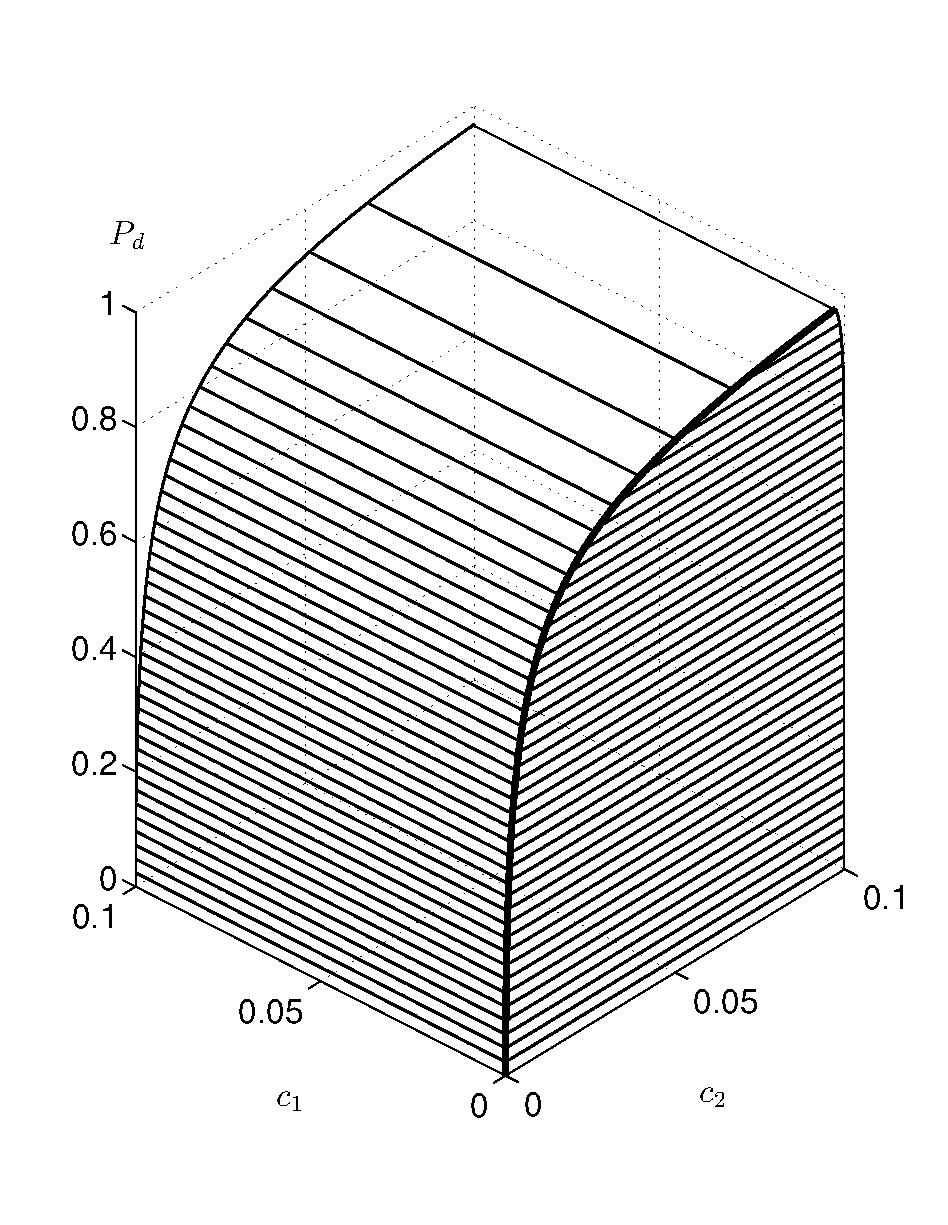
\includegraphics[width=12cm, height=16cm]{4/energy.eps}
\caption{M-ROC surface for $\sigma_\omega^2 = 0.1$, $\sigma_{s_1}^2=0.05$, $\sigma_{s_3}^2=0.15$ and $N = 20$.}
\label{pic:1201a1}
\end{figure}



%----------------------------------------------------------------------------------------------




%==========
\typeout{}
\chapter{Conclusions}
In this thesis, we explore the field of spectrum sensing for cognitive wireless communication, with aim of providing different levels of protections for various primary users. The necessary condition for ENP lemma (\rmnum{2}), under certain constraints are provided. We also show that under ENP test the normal direction for a specific point on the ROC surface can be represented by its associated ENP parameters. Furthermore, the relationship between the ENP test and a Bayesian test are discussed. 
A detector based on the ENP test can ensure the largest probability of detecting a free channel under separate constraints of false alarm  for each primary user type. However, with an ENP detector, the achievable false alarm probabilities are limited.  
In this thesis, we proposed the MENP framework which could achieve the largest probability of detection detection under multiple constraints of probability of false alarms under certain conditions. Two methods for finding the MENP parameters are provided. 
After that, we considered the M-ROC surface to represent the relationship between the probability of detection and the constraints. A sufficient condition under the ROC surface of the ENP test with positive parameters degenerates to a curve is provided.  Two examples concerning Gaussian distribution and Chi-Square distribution are given to show the properties of M-ROC surface.

We applied the new hypotheses testing framework to spectrum sensing in cognitive radio. The energy detector and cyclostationary detector are proposed to detect two primary users. Numerical results are provided for both detectors. It has also been proved that for any false alarm constraints, the energy detector can compute the decision rule under MENP framework easily. For cyclostationary detector, there is no direct relationship between the false alarm constraints and the MENP decision rule parameters. In such case, we need to use Qian's algorithm or look-up table method to acquire the MENP decision rule parameters. Both numerical results show that the probability of detection is non-decreasing with respect to the probabilities of false alarm constraints. However, lose the probability of false alarm constraint may not improve the probability of detection. A secure method to increase the probability of detection is checking the system's M-ROC surface and choose a proper probability of false alarm constraints.  

The simulation results for energy detector and cyclostationary detector are provided. In both simulations, we considered the relationship between $P_{f_1}$, $P_{f_2}$, $P_d$, $c_1$, $c_2$ and the MENP parameters.  A comparison between the numerical results and the simulation results are conducted. We can see the simulation results accords with the numerical results, which verify our theoretical analysis. 


%========== Appendices
\appendix

%==========
\typeout{}
\resetdatestamp

\chapter{Numerical Results Program Guide}
\label{A:LaTeXmacros}

%\section{}
This section explains how to use the Matlab code that was developed to generate the numerical results in this thesis.  The following table provides an overview of each source code file. All of these files can be found on the attached CD. 

\begin{table}[h]
\begin{tabular}{l|p{350pt}}
\hline
\hline
Source File Name                  & Description                                                                \\ \hline
gau\_roc.m      & Compute ROC for general Gaussian situation.              \\
QZ\_Algorithm.m & Implements algorithm proposed in \cite{zhang2000efficient} to get MENP parameters.                \\
gau\_equvar.m   & Compute MROC for Gaussian distributions with equal variances. \\
general\_gau.m         & Compute MROC for general Gaussian situations.                   \\
mychisquare.m            & Compute MROC for Chi-Square situation.                        \\
cycloPDFs.m              & Compute PDFs for cyclostationary detection.                 \\ 
general\_pdfs.m           & Compute MROC for given PDFs.                                 \\
cyclo.m				     & Compute MROC for cyclostationary detection.             \\		
plotfigure.m             & Plot ROC or MROC figure. \\
init.txt                   & Record the adjustable parameters for above programs.         \\
\hline
\end{tabular}
\label{filelist}
\caption{Matlab source files}
\end{table}

To run a program, all of the files in Table A.1 must be placed in the Matlab current work folder. These programs have been successfully run using Matlab 2013b and Matlab 2014a on Linux platform with 12 GB RAM.  
To generate ROC surface for a Gaussian case, run gau\_roc.m. This can be done by running the following command in Matlab command line.
\\\texttt{Matlab$>$ gau\_roc}

The file loads configurations from init.txt file. When the computation finishes file gau\_roc.mat stores the results and plotfigure.m excutes automatically to print the ROC surface on the screen.


To generate the M-ROC surface for general Gaussian case, run general\_gau.m. This can be done by running the following command in Matlab command line.
\\\texttt{Matlab$>$ genaral\_gau}

The file loads configurations from init.txt file. When the computation finishes file general\_gau.mat stores the results and plotfigure.m excutes automatically to print the MROC surface on the screen.


To generate the M-ROC surface for the Gaussian case with equal variance, run gau\_equvar.m. This can be done by running the following command in Matlab command line.
\\\texttt{Matlab$>$ gau\_equvar}

The file loads configurations from init.txt file. When the computation finishes the file gau\_equvar.mat stores the results and plotfigure.m excutes automatically to print the MROC surface on the screen.

To generate the M-ROC surface for Chi-Square situation, run mychisquare.m. This can be done by running the following command in Matlab command line.
\\\texttt{Matlab$>$ mychisquare}

The file loads configurations from init.txt file. When the computation finishes file mychisquare.mat stores the results and plotfigure.m excutes automatically to print the MROC surface on the screen.

To generate the M-ROC surface cyclostationary detection, run cyclo.m. This can be done by running the following command in Matlab command line.
\\\texttt{Matlab$>$ cyclo}

The file loads configurations from init.txt file. When the computation finishes file PDFs.mat stores the PDFs for each hypothesis and  cyclo.mat stores the MROC data.

To compute MENP parameters for specific false alarm constraints, run QZ\_Algorithm.m with the false alarm constraints as arguments. This can be done by running following command in Matlab command line.
\\\texttt{Matlab$>$ QZ\_Algorithm(c1, c2)}

After the computation, the program prints the MENP parameters on the screen. 

The adjustable parameters for ENP (MENP) test are recorded in init.txt file and listed in Table A.2. 
\begin{table}[h]
\begin{tabular}{l|p{350pt}} 
\hline
\hline
Constant Name & Description                                                                                           \\
\hline
STEP\_K       & Step of ENP parameters, should be positive                                                            \\
RANGE\_K      & Range of ENP parameters, should be positive                                                           \\
MU0		  &  Mean of hypothesis $H_0$.\\
MU1		  & Mean of hypothesis $H_1$.\\
MU2       & Mean of hypothesis $H_2$.\\
VAR0      &    Variance of hypothesis $H_0$.\\
VAR1		&	Variance of hypothesis $H_1$.\\
VAR2		&		Variance of hypothesis $H_2$.\\
CHI\_DEGREE   & Degree of freedom in Chi-Square Example. Should be a positive integer.                                \\
DA\_LEN       & The length of data of OFDM. Should be an positive integer.                      \\
CP\_LEN       & The length of CP of OFDM. Should be an positive integer and smaller than DA\_LEN. \\
FRAME\_NUM    & The number of received OFDM frames. Should be an positive integer.\\
\hline                                   
\end{tabular}
\label{constantlist}
\caption{Adjustable Constants}
\end{table}



%========== Bibliography
\typeout{}
\begin{singlespace}
  \bibliography{ThesisEx}
  \bibliographystyle{ieeetr}
\end{singlespace}

\end{document}
